%!TEX root = ../aluno.tex

\ifnum\aluno=1
\renewcommand\chapterillustration{./abertura-investigacao}
\else
\renewcommand\chapterillustration{./abertura-investigacao-professor}
\fi

\def\chapterwhat{Taxas, índices e indicadores sociais, econômicos e ambientais. Compreensão de aspectos teóricos e práticos dessas informações, com uma metodologia que busca a análise de situações reais, tanto locais quanto globais.}

\def\chapterbecause{Na era da informação, somos inundados por dados sobre os mais diversos fenômenos da realidade. Compreender a obtenção e organização desses dados torna-se importante para planejarmos ações que busquem uma organização social mais justa e sustentável.} 
\chapter{Projetos de Investigação com Matemática}
\label{ladri-chap}

\mbox{}\thispagestyle{empty}\clearpage

\thispagestyle{empty}

\begin{center}
Projeto: LIVRO ABERTO DE MATEMÁTICA

\noindent \begin{tabular}{lcccr}

\includegraphics[scale=.15]{impa}& \quad\quad& 
\includegraphics[width=3cm]{logo} & \quad\quad& 
\includegraphics[scale=.24]{obmep} 
\end{tabular}
\end{center}

\vspace*{.3cm}

Cadastre-se como colaborador no site do projeto: \url{umlivroaberto.org}


% \begin{center}
%   \includegraphics[width=2cm]{canvas}
% \end{center}

\begin{tabular}{p{.15\textwidth}p{.7\textwidth}}
Título: & Projetos de Investigação com Matemática\\
\\
Ano/ Versão: & 2020 / versão 0.2 de \today\\
\\
Editora & Instituto Nacional de Matem\'atica Pura e Aplicada (IMPA-OS)\\
\\
Realização:& Olimp\'iada Brasileira de Matem\'atica das Escolas P\'ublicas (OBMEP)\\
\\
Produção:& Associação Livro Aberto\\
\\
Coordenação: & Fabio Simas, \\
			&  Augusto Teixeira (livroaberto@impa.br)\\
\\
  Autor: & Thiago Ferraiol, \\
         & Priscila Santos, \\
         & Rodrigo Belli \\
\\
Revisor: &  Letícia Rangel  \\
\\
Design: & Andreza Moreira (Tangentes Design) \\
\\
  Ilustrações: & --- \\ 
\\
Gráficos: & --- \\
\\
  Capa: & Foto de Clay Banks, no Unsplash \\
  		& https://unsplash.com/photos/U0-r0JMypE0 \\

\end{tabular}


\begin{figure}[b]
\begin{minipage}[l]{5cm}
\centering

{\large Licença:}

  
\includegraphics[width=3.5cm]{cc-by-nc-sa}
\end{minipage}\hfill
\begin{minipage}[c]{5cm}
\centering
{\large Desenvolvido por}


\includegraphics[width=2.5cm]{logo-associacao.jpg}
\end{minipage}
\begin{minipage}[r]{5cm}
\centering

{\large Patrocínio:}
  \vspace{1em}
  
\includegraphics[width=3.5cm]{itau}
\end{minipage}
\end{figure}

\mainmatter

\begin{apresentacao}{Introdução}
\subsection{Para começo de conversa}

Este capítulo é um convite à experiência de uma nova forma de trabalhar em sua sala de aula. A proposta aqui é possibilitar que os estudantes se aprofundem em perguntas próprias, por meio de uma metodologia de investigação que será guiada por você. A temática da pandemia causada pelo novo coronavírus será utilizada durante todo o capítulo como exemplo de projeto, de forma a dar mais concretude à proposta. A escolha da metodologia de trabalho como foco do capítulo tem o objetivo de abrir a possibilidade para que você e seus estudantes escolham uma temática que julguem importante e interessante para a comunidade escolar na qual estão inseridos. A intenção é propor uma sequência didática que seja interessante e cativante para cada estudante, mas que também possibilite que eles experimentem utilizar seus conhecimentos matemáticos para refletir sobre a sociedade e desenvolvam estratégias para agir sobre ela. Pois, para que o estudante torne-se capaz de utilizar as ferramentas matemáticas para interpretar fatos de forma crítica, é necessário que ele experimente como fazer isso. 

Dan Meyer, pesquisador da área da educação matemática, defende que uma atividade será cativante e interessante para os estudantes se eles puderem propor suas próprias perguntas de investigação \citep{meyer2011}. Ao mesmo tempo, Jo Boaler, outra pesquisadora da área, defende que o aprendizado é mais interessante e mais efetivo quando os estudantes podem trabalhar de forma investigativa, com problemas abertos que possibilitem o emprego da criatividade, do trabalho coletivo, das discussões de ideias e da diversidade das formas de se pensar e resolver problemas \citep{boaler2018}.

Já pesquisadores como Olé Skovsmose, Eric Gutstein, Bob Peterson e Marilyn Frankenstein entre outros, defendem que é necessário que parte do trabalho nas aulas de matemática seja dedicado a olhar e compreender os problemas da sociedade a partir das ferramentas que o aprendizado da matemática proporciona, ajudando o estudante a entender como utilizá-las em contextos da realidade individual de cada um (ou de cada comunidade escolar), para dar sentido ao mundo que o cerca \citep{skovsmose2014,gutstein2013,frankenstein2014}.

Uma inspiração para a elaboração dessa proposta são as atividades elaboradas pelo Programa Nossa Escola Pesquisa Sua Opinião (Nepso). Utilizando as pesquisas de opinião como ferramenta pedagógica, sua metodologia consiste na formação de grupos de trabalho que, independente da temática, são norteados pela construção da autonomia dos estudantes, pela compreensão de seu contexto e consequente engajamento \citep{andrade2014}.

A abordagem metodológica proposta neste capítulo pode ser enquadrada dentro do que é chamado de pelos pesquisadores da área de Metodologia de Investigação Matemática, que tem sido largamente debatida e incentivada, já a algumas décadas. Algumas referências do tema são \citet*{ponte2019} e \citet{dambrosio1993}. 

\columnbreak

\subsection{Habilidades da BNCC trabalhadas neste capítulo}
\begin{habilities}{EM13MAT101}
Interpretar criticamente situações econômicas, sociais e fatos relativos às Ciências da Natureza que envolvam a variação de grandezas, pela análise dos gráficos das funções representadas e das taxas de variação, com ou sem apoio de tecnologias digitais.

\tcbsubtitle{EM13MAT102}
Analisar tabelas, gráficos e amostras de pesquisas estatísticas apresentadas em relatórios divulgados por diferentes meios de comunicação, identificando, quando for o caso, inadequações que possam induzir a erros de interpretação, como escalas e amostras não apropriadas. 

\tcbsubtitle{EM13MAT103}
Interpretar e compreender textos científicos ou divulgados pelas mídias, que empregam unidades de medida de diferentes grandezas e as conversões possíveis entre elas, adotadas ou não pelo Sistema Internacional (SI), como as de armazenamento e velocidade de transferência de dados, ligadas aos avanços tecnológicos. 

\tcbsubtitle{EM13MAT104}
Interpretar taxas e índices de natureza socioeconômica (índice de desenvolvimento humano, taxas de inflação, entre outros), investigando os processos de cálculo desses números, para analisar criticamente a realidade e produzir argumentos.

\tcbsubtitle{EM13MAT202}
Planejar e executar pesquisa amostral sobre questões relevantes, usando dados coletados diretamente ou em diferentes fontes, e comunicar os resultados por meio de relatório contendo gráficos e interpretação das medidas de tendência central e das medidas de dispersão (amplitude e desvio padrão), utilizando ou não recursos tecnológicos.
\end{habilities}

Além das habilidades descritas, o capítulo trabalha a competência específica nº 2, da área de Matemática:

“Propor ou participar de ações para investigar desafios do mundo contemporâneo e tomar decisões éticas e socialmente responsáveis, com base na análise de problemas sociais, como os voltados a situações de saúde, sustentabilidade, das implicações da tecnologia no mundo do trabalho, entre outros, mobilizando e articulando conceitos, procedimentos e linguagens próprios da Matemática.”

A partir dele, também são desenvolvidas três competências gerais da educação básica, descritas na BNCC. São elas:

\begin{habilities}{Competência geral 1}
Valorizar e utilizar os conhecimentos historicamente construídos sobre o mundo físico, social, cultural e digital para entender e explicar a realidade, continuar aprendendo e colaborar para a construção de uma sociedade justa, democrática e inclusiva. 

\tcbsubtitle{Competência geral 2}
Exercitar a curiosidade intelectual e recorrer à abordagem própria das ciências, incluindo a investigação, a reflexão, a análise crítica, a imaginação e a criatividade, para investigar causas, elaborar e testar hipóteses, formular e resolver problemas e criar soluções (inclusive tecnológicas) com base nos conhecimentos das diferentes áreas.

\tcbsubtitle{Competência geral 5}
Compreender, utilizar e criar tecnologias digitais de informação e comunicação de forma crítica, significativa, reflexiva e ética nas diversas práticas sociais (incluindo as escolares) para se comunicar, acessar e disseminar informações, produzir conhecimentos, resolver problemas e exercer protagonismo e autoria na vida pessoal e coletiva.
\end{habilities}

\subsection{Proposta metodológica}
A \hyperref[etapas-metodologicas]{proposta deste capítulo} está calcada em cinco pontos, cada um indicando um momento das atividades no ambiente escolar que levam do cotidiano à abstração, retornando em seguida ao cotidiano, então numa outra condição.

% \begin{figure}[H]
% \centering
% 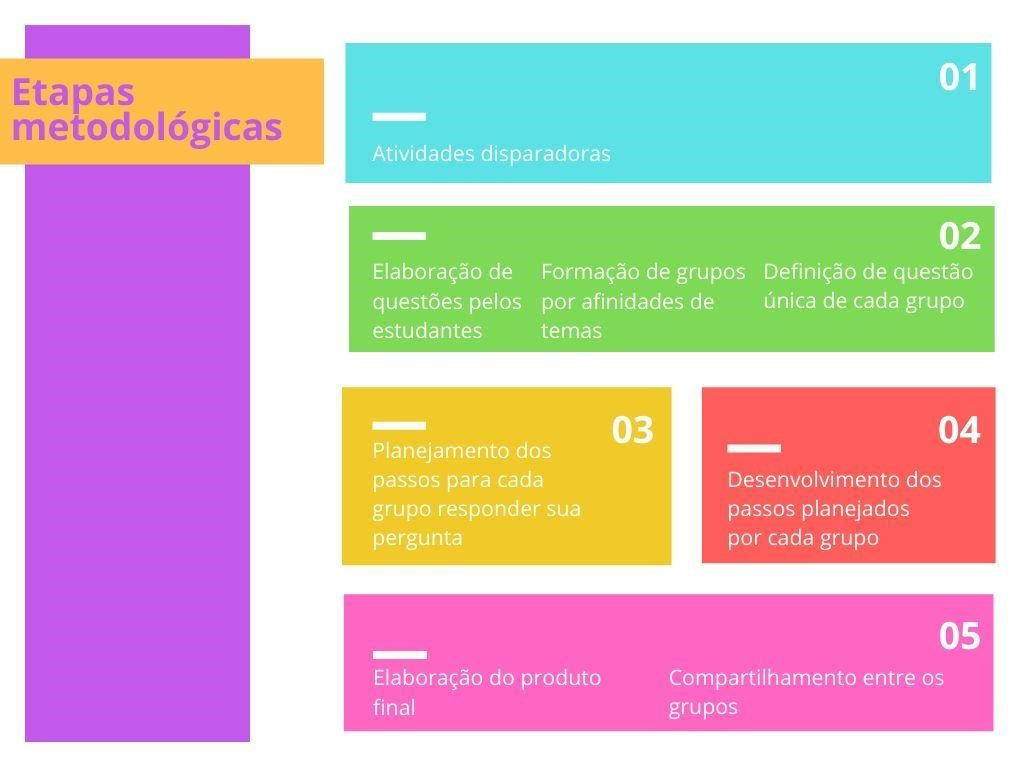
\includegraphics[width=\linewidth]{investigacao1.jpg}

% \end{figure}

A primeira etapa da metodologia está no \hyperref[etapa1]{\textcolor{session1}{\textbf{Explorando: Atividades disparadoras - Etapa 1}}}. Nela o educador deve oferecer materiais sobre a temática do projeto, ou instruir os estudantes sobre como obtê-las. Sua razão de ser está na intenção de que os estudantes se aproximem da temática a ser trabalhada. Em propostas de modelagem matemática, ela costuma ser a discussão de um problema da comunidade. Entretanto é possível partir de qualquer temática. Elas podem ser compostas por textos e/ou vídeos jornalísticos, por materiais artísticos (como poesia, contos, crônicas, apresentações, instalações, performances), por relatórios e artigos científicos, por depoimentos dos próprios estudantes ou de pessoas da comunidade escolar. Qualquer recurso é válido desde que as atividades disparadoras permitam o professor auxiliar os estudantes no exercício inicial de entendimento do contexto em que vivemos.

Sobre o significado do termo "contexto em que vivemos"{}, cabe dizer que aqui ele não é entendido de forma estática, restrito aos limites da vida imediata. O contexto de vida de cada um se transforma na medida em que novas situações e ideias se apresentam e se incorporam à nossa práxis, ou seja, na relação dialética entre teoria e prática. Nesse sentido, é entendido que a escola tem o papel fundamental de ampliar os contextos com os estudantes, trazendo novas situações da realidade e, ao mesmo tempo, criando uma conexão com o cotidiano, gerando a necessidade de questionar e agir de forma crítica.

Segue-se às atividades disparadoras a segunda etapa, que se encontra na seção \hyperref[etapa2]{\textcolor{session1}{\textbf{Explorando: Elaboração de questões - Etapa 2}}}. Nela, cabe ao professor auxiliar os estudantes na organização de suas atividades de trabalho. Dentro da perspectiva didática de sair do concreto ao abstrato, é preciso encontrar na dimensão cotidiana problemas que incitem a pesquisa. Elaborar questões, portanto, é imprescindível. Mas não se trata de qualquer tipo de questão. Considerando a familiaridade dos estudantes à prática científica, o tempo disponível à realização das atividades e a infraestrutura escolar ofertada, as questões devem respeitar alguns limites. Estes seriam:

\begin{itemize}
\item apresentar caráter quantitativo, dado que a proposta será realizada em aulas de matemática;

\item exequíveis nas condições estabelecidas pelo ambiente escolar e pela dinâmica da disciplina;

\item devem ser comparativas, restringindo o escopo de questões, mantendo-as menos abrangentes;

\item interessantes, de forma que não sejam respondidas com uma busca simples na internet;

\item simplicidade, isto é, apresentar pretensões modestas.
\end{itemize}

Após a elaboração das questões é hora de formar os grupos de trabalhos. Os componentes do grupo devem acordar sobre um único problema, ou seja, uma única questão a ser tratada, dividindo as tarefas necessárias para seu estudo e se atentando para a revisão daquilo que foi produzido por seus colegas.

Escolhidas as questões por cada grupo, chega-se à terceira etapa que se encontra na seção \hyperref[etapa3]{\textcolor{session4}{\textbf{Organizando: Planejando a investigação - Etapa 3}}}. Aqui, a partir dos problemas colocados, os estudantes deverão se aprofundar nas ferramentas necessárias para a execução da pesquisa. Considerando as características limitadoras das questões, as possibilidades de aprofundamento deverão atinar sobre quais seriam os principais indicadores relacionados ao tema estudado. Devem também reconhecer quais os dados necessários para responder à questão e de onde será possível extraí-los. Nesse sentido, valerá a pena identificar quais as fontes de dados confiáveis. E, também, como proceder metodicamente sobre os dados a partir das ferramentas selecionadas, tal como um projeto de pesquisa acadêmica.

Definido o projeto, torna-se possível partir para a seção \hyperref[etapa4]{\textcolor{session2}{\textbf{Praticando: Desenvolvendo a investigação - Etapa 4}}}. Nela, os estudantes efetivamente utilizarão os novos conhecimentos e provavelmente adquirirão mais alguns. É nesta fase do trabalho que os conceitos e categorias apreendidos no momento anterior serão realmente aplicados, ganhando profundidade. Cabe ao educador, nesta quarta etapa, abordar junto aos estudantes os conceitos como os tipos de gráfico e seus usos, como calcular taxas, razões e porcentagens, e demais ferramentas necessárias para a conclusão da pesquisa.

É importante que você, educador ou educadora, oriente os estudantes desde o início do projeto sobre a necessidade de elaboração de um produto final. Nesta quinta e última etapa, que se encontra na seção \hyperref[etapa5]{\textcolor{session2}{\textbf{Praticando: Comunicando as descobertas - Etapa 5}}}, o estudante efetivará a pesquisa trabalho de análise matemática apresentando um produto final que compartilhe seus resultados com todos os colegas da comunidade escolar.

Este produto pode apresentar variadas formas. Algumas possibilidades são:
\begin{itemize}
\item uma revista “científica” com os artigos dos grupos;
\item um congresso com um seminário de cada “grupo de pesquisa”;
\item uma série de podcasts, no qual cada grupo faz o seu programa;
\item um telejornal ou um canal com vídeos de cada grupo;
\item uma página de internet para cada grupo apresentar suas descobertas sobre o tema estudado;
\item um fanzine ou uma história em quadrinhos (HQ);
\item um panfleto ou um folder.
\end{itemize}

Lembre-se que o produto final permite uma verificação mais aprofundada sobre o processo de pesquisa científica do estudante desde que este saiba desde o início qual deve ser o seu objetivo. O produto, independente da forma materializada, orienta as ações no decorrer das atividades e, quando finalizado, permite o escrutínio das etapas percorridas.

Ainda sobre os produtos conclusivos das pesquisas, é preciso destacar qual deve ser a força de suas considerações finais. Em outras palavras, o que se espera alcançar ao final, considerando o ponto de vista avaliativo. Ao estarem limitadas ao cotidiano dos estudantes, devem servir muito mais como um estímulo à pesquisa científica e ao exercício da intervenção prática sobre a realidade a partir de sua objetividade do que um grande aprofundamento abstracionista. Mais do que responder à questões especulativas, devem verificar problemas de qualquer natureza em seu contexto para, enfim, propor soluções. Indubitavelmente, o conhecimento socialmente produzido não pode ser ignorado. As considerações alcançadas pelos estudantes não podem deixar de ser confrontadas com aquilo que é realizado atualmente, de uma maneira muito mais vigorosa e consequente, dentro do ambiente acadêmico.

Ao longo da proposta de montagem de um itinerário de pesquisa é apresentado a você, detalhadamente, como cada etapa pode ser elaborada. Existem aspectos indispensáveis a serem levados em consideração caso não se queira reproduzir a didática  conteudista comum nas disciplinas escolares.

Todo esse percurso foi pensado para ser desenvolvido em um mês de atividades (com base em um curso de matemática com 5 aulas de 50 minutos por semana). Sugerimos a seguinte distribuição destas aulas: 

\begin{itemize}
\item 2-3 aulas para a atividade disparadora
\item 2-3 aulas para a elaboração das questões de investigação
\item 4-5 aulas para a elaboração do planejamento 
\item 7-8 aulas para o desenvolvimento da investigação
\item 4-5 aulas para a produção do produto final e compartilhamento
\end{itemize}

Ter mais ou menos tempo para dedicar a cada etapa define a complexidade e profundidade das questões investigativas e das análises que os estudantes podem propor.

\subsection{Avaliação}

Em qualquer processo avaliativo é muito importante ter em mente o que se quer avaliar. O principal objetivo deste capítulo é ensinar os estudantes a buscarem autonomamente respostas quantitativas sobre problemas de cunho econômico, social ou ambiental e interpretarem criticamente as informações obtidas por meio da análise dos processos de cálculo de taxas, índices e razões. Assim, é importante avaliar:

\begin{itemize}
\item o desenvolvimento da autonomia dos estudantes na busca por respostas de questões relativamente complexas;
\item a compreensão do que são taxas, índices e razões;
\item a apropriação da matemática envolvida nos cálculos de taxas, índices e razões;
\item como esse conhecimento pode ser utilizado criticamente.
\end{itemize}

A avaliação aqui é compreendida como um processo formativo, que pode ser entendido como instrumento de caráter pedagógico, regulador \citep{sanmarti2009}. Nesse entendimento, os instrumentos avaliativos têm o objetivo de identificar mudanças que necessitam ser introduzidas no processo de ensino, de forma a ajudar os estudantes em seu próprio processo de construção de conhecimento. 

Toda a proposta deste capítulo tem a ver com os estudantes terem a oportunidade de buscarem caminhos próprios, individuais em alguma medida, de forma a tornarem-se mais autônomos, se verem como produtores de conhecimento e agentes de mudança da sociedade. É importante que o processo avaliativo reflita estas ideias e seja instrumento que ajude no desenvolvimento desta autonomia. 

Dentro dessa perspectiva, é recomendável que o processo avaliativo seja realizado a partir dos materiais elaborados pelos próprios estudantes ao longo de todo o percurso do capítulo e de atividades de autoavaliação e reflexão sobre os percursos individualizados. 

Os materiais produzidos pelos estudantes são: 
\begin{itemize}
\item As perguntas (na 2\super{a} etapa);
\item Um planejamento em grupo, na 3\super{a} etapa, que mostrará a interpretação inicial dos estudantes sobre os índices e taxas, assim como uma hipótese a ser averiguada e uma proposta de operações e análises.
\item Ao final da 4\super{a} etapa o estudante responderá individualmente uma série de questões que, ao serem comparadas com seu planejamento inicial, poderá mostrar uma evolução da compreensão sobre o emprego de taxas e índices na análise de situações do mundo real. Este material também possibilitará o educador a perceber o quanto o estudante se apropriou dos métodos utilizados pelo seu grupo para realizar as análises de dados. 
\item O produto final, resultado da 5\super{a} etapa desta metodologia, é a concretização do uso social da matemática trabalhada durante todo o capítulo e também pode ser avaliado.
\end{itemize}

A avaliação formativa se dá na comparação dos instrumentos produzidos nas etapas 2 e 3 com aqueles produzidos nas etapas 4 e 5. A partir dessa comparação é possível avaliar a evolução do estudante quanto às estratégias utilizadas, aos sentidos dados para taxas, índices e razões, aos cálculos realizados e à utilização dessas informações para justificar opiniões e pensar em ações concretas para a mudança da realidade. 

Já as autoavaliações têm papel fundamental no processo de desenvolvimento de autonomia e auto regulação para o estudo. Uma possibilidade é inserir atividades de autoavaliação no meio das etapas 3, 4 e 5 ou ao final delas. Alguns exemplos de autoavaliação estão no \hyperref[avaliacoes]{final deste capítulo}

Se o educador sentir falta de um instrumento individual de avaliação, uma possibilidade é propor a produção de um relatório individual ao final da 4ª ou da 5ª etapa, com o objetivo de evidenciar os aprendizados individuais. Uma possibilidade de roteiro para um relatório individual também está presente no\hyperref[relatorio-individual]{final do capítulo}

\subsection{Considerações finais}

A metodologia proposta se apresenta como um guia para as atividades em sala de aula, sendo verificável apenas no momento de sua aplicação. Por isso, a equipe do Livro Aberto conseguirá ter melhores condições de avaliação da proposta a partir do retorno da sua atividade. Pedimos que entre em contato para compartilhar suas experiências e projetos realizados a partir do livro. Assim, será possível construir um inventário bastante volumoso de exemplos e práticas que apontam os limites e as possibilidades da utilização dessa metodologia.

Por último, lembre-se que o desenvolvimento desta unidade é um convite a interdisciplinaridade. Compartilhe suas ideias com seus colegas de outras áreas e convide-os para construir o projeto com você.

\subsection{Leituras de aprofundamento}

Sobre as características de nosso período conjuntural, de expansão das tecnologias da informação e da comunicação a sua predominância na organização de nossas vidas, confira \citep{castells1999}.

Sobre o significado e o proceder da análise de conjuntura, confira \citep{souza2012}.

\end{apresentacao}

\explore{Para começo de conversa}

As análises sobre a realidade social precisam se atentar àquilo que os especialistas chamam de conjuntura (Você Sabia: O que é conjuntura?). Nossa conjuntura compreende o período que se inicia a partir da segunda metade do século XX. Em nossa época, ocorre a terceira revolução industrial, também chamada de revolução microeletrônica ou digital. Essa revolução é caracterizada pela passagem de processos mecânicos e analógicos para processos digitais.

A partir do final do século XX deu-se também a massificação do uso dos computadores e da internet, permitindo que nos comuniquemos instantaneamente e inundando nosso mundo de informações. Este período mais recente representa uma quarta fase do desenvolvimento industrial, o da revolução 4.0, momento em que as tecnologias da informação e da comunicação estão completamente integradas em rede com outras dimensões da vida, operando instantaneamente à distância (SCHWAB, 2016). Por isso nossa conjuntura é conhecida por alguns como a era da informação.

No entanto, ao contrário do que poderíamos imaginar, quanto maior o fluxo de informações que nos chega, mais parecemos incapazes de interpretá-las. Entramos em um aparente paradoxo: percebemo-nos seres com cada vez mais informações e, ao mesmo tempo, cada vez menos informados. Existem algumas explicações para esse aparente paradoxo. Uma delas, dada pelo sociólogo polonês Zygmunt Bauman (2001), é que as informações na modernidade, da mesma forma que a produção e as relações sociais, estão cada vez mais líquidas. Isto significa que, assim como a água, elas se movem e se transformam muito rapidamente, dificultando nossa tarefa de sintetizá-las e utilizá-las objetivamente para interpretar o mundo e tomarmos decisões coletivas. Esse contexto de fartura, aliada à fragmentação, nos traz mais confusão do que formação, restringindo nossas ações aos aspectos individuais (daí a liquidez também manifestada nas relações sociais).

Neste sentido, o saber matemático pode se tornar uma ferramenta indispensável à análise sociológica, já que boa parte dessas informações pode ser medida, quantificada e traduzida em dados estatísticos. Assim, esses dados expressam, através dos números, dos índices, das tabelas e dos gráficos, partes das nossas condições atuais, das transformações ocorridas no mundo e servem de parâmetros para pensarmos em novas perspectivas de vida e de desenvolvimento.

Mas como podemos fazer isso? Afinal, se considerarmos o argumento de Bauman, nossa própria realidade social dificultaria o exercício de avaliação.

A chave para quebrarmos a reprodução desse entendimento está em partirmos do cotidiano - de suas expressões mais imediatistas - ao abstrato - as formulações pretensamente mais gerais -, e retornamos ao cotidiano numa nova condição, confrontando-o ao conhecimento socialmente construído pela prática científica.

\subsection{Proposta metodológica}

A proposta deste capítulo está calcada em cinco pontos, cada um indicando um momento das atividades no ambiente escolar que levam do cotidiano à abstração, retornando em seguida ao cotidiano, já numa nova condição

\begin{figure}[H]
\phantomsection\label{etapas-metodologicas}
\centering
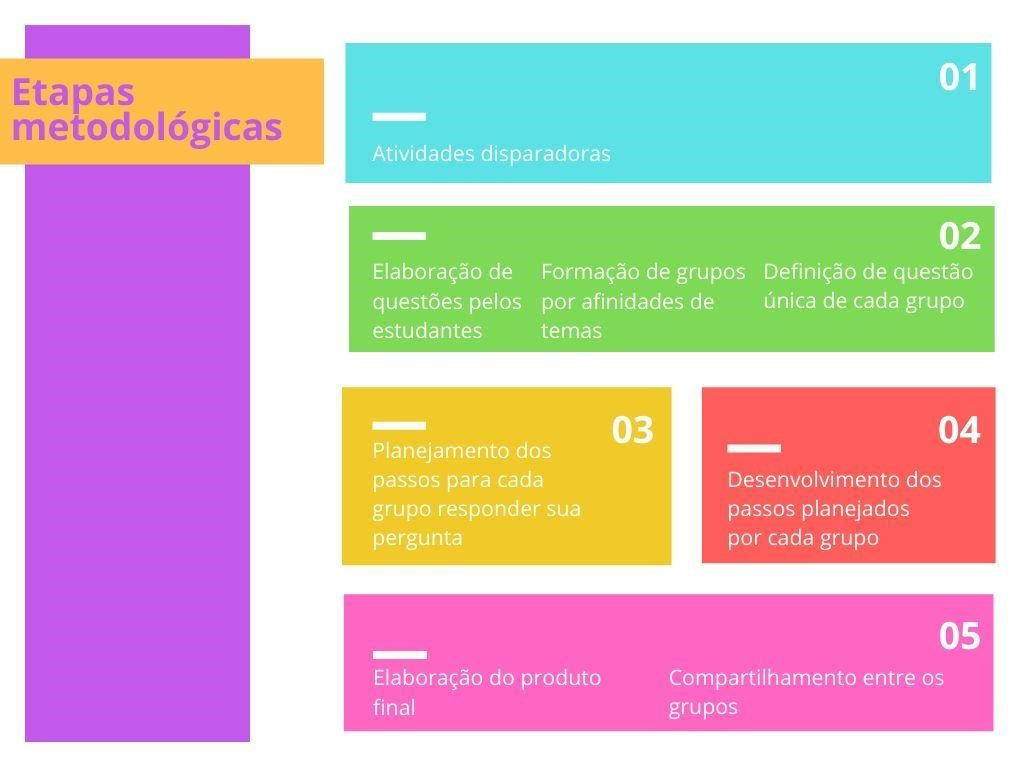
\includegraphics[width=350bp]{investigacao1.jpg}

\end{figure}

\begin{itemize}
\item \hyperref[etapa1]{\textcolor{session1}{\textbf{Explorando: Atividades disparadoras - Etapa 1}}}: Etapa para conhecer materiais que lhe provoquem um estranhamento (Para saber +: O cotidiano e seu estranhamento) daquilo que acontece em sua rotina e lhe permita iniciar questionamentos sobre ela. São materiais como textos e/ou vídeos jornalísticos, materiais artísticos (como poesia, contos, crônicas, apresentações, instalações, performances), depoimentos de seus colegas ou de outras pessoas da comunidade escolar, etc. Estes materiais serão fornecidos por seu professor ou indicado por ele como acessá-los.

\item \hyperref[etapa2]{\textcolor{session1}{\textbf{Explorando: Elaboração de questões - Etapa 2}}}: Tem o objetivo de organizar as questões provenientes das atividades disparadoras em um problema geral que permita uma análise objetiva a partir do uso de indicadores. Além disso, serão formados grupos de trabalho, no qual cada um terá a sua questão investigativa.

\item \hyperref[etapa3]{\textcolor{session4}{\textbf{Organizando: Planejando a investigação - Etapa 3}}}: A partir dos problemas colocados, você e seus colegas deverão se aprofundar nas ferramentas necessárias para a execução da pesquisa. Esta é a terceira etapa da metodologia proposta.

\item \hyperref[etapa4]{\textcolor{session2}{\textbf{Praticando: Desenvolvendo a investigação - Etapa 4}}}: Nesta quarta etapa você e seus colegas utilizarão novos conhecimentos, construídos nas etapas anteriores, e provavelmente adquirirão mais alguns. É nesta fase do trabalho que os conceitos apreendidos no momento anterior serão realmente aplicados, ganhando profundidade. 

\item \hyperref[etapa5]{\textcolor{session2}{\textbf{Praticando: Comunicando as descobertas - Etapa 5}}}: Nesta quinta e última etapa cada grupo deve apresentar a pesquisa de análise matemática em um formato concreto, compartilhando seus resultados com todos os colegas da comunidade escolar.
\end{itemize}

Ainda sobre os produtos conclusivos das pesquisas, o que se espera alcançar ao final é um estímulo à pesquisa científica e ao exercício da intervenção prática sobre a realidade a partir de sua objetividade.

Todas as etapas de desenvolvimento do projeto serão apresentadas nas próximas seções por meio de um exemplo, que utiliza a pandemia do novo coronavírus para dar concretude às propostas de atividades e reflexões.

\know{O cotidiano e seu estranhamento}

De acordo com a filósofa húngara Agnes Heller, nossas vidas são marcadas profundamente pela dimensão do cotidiano. Como o próprio nome sugere, trata-se do momento da vida que nos ocupamos com nossa rotina diária. Quanto mais o tempo passa e, consequentemente, mantemos os elementos essenciais da rotina intocados, mais nos acostumamos a tratar tudo aquilo que nos acontece como algo “natural”, como algo que não possuísse outra alternativa de ser.

Mas a natureza, assim como a vida social, é bastante dinâmica. Basta prestarmos atenção ao nosso redor para identificarmos, tanto na natureza quanto na sociedade, formas bastante diferentes de manifestação da vida. Neste momento, podemos realizar um exercício de estranhamento, ou seja, de questionamento daquilo que está estabelecido e de proposição de algo diferente do corriqueiro. Deste modo surgem as diversas formas de arte, de ciência e de política. Todas criações humanas que ganham autonomia relativa diante da dimensão cotidiana.

\begin{knowledge}{O que isso, a conjuntura?}

O termo conjuntura se tornou recorrente na historiografia recente graças à figura de Fernand Braudel. Historiador francês vinculado à escola dos Annales, ele foi responsável por propor outro modelo de registro da  história.

De uma disciplina atrelada aos estudos do passado, que buscava cada vez mais compreender o chamado tempo presente, \citeauthor{braudel1978} vincula seu ofício a uma forma de compreensão mais ampla, agregando recursos de análise das ciências humanas em geral.

De maneira bem resumida, para \citeauthor{braudel1978}, seria possível realizar uma pesquisa historiográfica a partir de três níveis: estrutural, conjuntural e fatual. No primeiro seria possível observar fenômenos de longa duração, relações sociais e ambientais dos seres humanos que permanecem ativos por longos períodos. No conjuntural, são os fenômenos de média duração, que não consolidam estruturas de relação, mas que não se resumem a meras acontecimentos pontuais, algo restrito ao entendimento da história fatual (aquela que se contenta, como o nome sugere, aos fatos, a imediaticidade das relações).

Portanto, quando nos referimos à conjuntura, estamos considerando uma forma de análise histórica que, sem ignorar os acontecimentos pontuais e as grandes estruturas de relações que permanecem ativas por longos períodos de tempo, se concentra em abordar o movimento. Em outras palavras, de que maneira os acontecimentos pontuais são expressão das grandes estruturas de sociabilidade e em que medida sua concretização abre caminhos para uma alteração nessa mesma estrutura.

\end{knowledge}

\begin{paginatexto}{Atividades disparadoras - Etapa 1}
\textit{(Tempo estimado 2-3 aulas)}

Vamos começar os trabalhos a partir dos temas disparadores. Como o próprio nome sugere, trata-se de atividades orientadas a partir de uma situação inicial propensa à problematização.

O objetivo dessa etapa é estimular o pensamento dos estudantes para formulação de perguntas a partir de situações comuns ao seu cotidiano, interrompendo a leitura naturalizante de seu contexto. Um segundo objetivo é iniciar o contato dos estudantes com o conceito de indicadores. Assim, as atividades disparadoras já devem trazer alguns índices ligados ao tema escolhido para o projeto. 

Os temas podem ser apresentados de variadas formas. Podem ser compilados na própria sala de aula, a partir de discussões regulares apresentadas pelos estudantes ao longo do ano letivo, como um acontecimento particular daquela turma. Podem ser também temas de repercussão em veículos de comunicação, como a situação política a nível institucional, a economia e seus desdobramentos no dia-a-dia da comunidade escolar, as questões ambientais mais importantes do momento ou a última moda cultural.

Com o avanço das tecnologias da informação e da comunicação, vale se aprofundar também nas discussões alçadas por influenciadores digitais. Existem conteúdos produzidos com o intuito de avaliar a realidade social que são capazes de alcançar corações e mentes dos estudantes.

Para exemplificar a metodologia foi escolhido um caso que seja vivenciado por um conjunto gigantesco de pessoas, mas de maneiras completamente diversas. Algo recorrente na história da humanidade, mas que sempre se apresenta sob novas formas: as crises civilizatórias.

O mundo que comporta um trânsito intenso de informações é também um mundo marcado pela circulação massiva de pessoas e mercadorias. Tal qual o evento das grandes navegações na metade do milênio passado, a expansão das relações humanas representa uma nova configuração territorial. Novas cidades surgem, velhas cidades se modificam, pessoas separadas por milhares de quilômetros se integram numa mesma relação.

Este conjunto de novas relações se desdobra em diversas consequências, capazes de erguer impérios como de derrubá-los. Do mesmo modo que a expansão da atividade econômica agrícola através da escravização consolidou o império romano, o expansão territorial desregrada e o contato de diversas culturas disseminou graves epidemias que contribuíram para a sua deterioração. Pois um dos pilares que sustentam qualquer formação social é a ideia de segurança sanitária não anormalidade na manutenção biológica da vida. Isso significa que toda a sociedade está em risco.

De tempos em tempos a humanidade vivencia grandes crises sanitárias, que afetam diferentemente os diversos territórios ocupados. Considerando nossa capacidade científica, quais são os motivos que nos impedem de evitá-las?

A pandemia causada pelo vírus SARS-CoV-2 pode exemplificar bem isso. Ela coloca em xeque o impacto do desenvolvimento urbano sobre a natureza e sobre a vida dos seres humanos. Também coloca em xeque a maneira como organizamos os nossos sistemas de saúde, para que possamos ter uma qualidade de vida para a população como um todo. E temos também uma crise de caráter da manutenção da produção e reprodução das condições de existência.

Perceba que a pandemia atua como um tema disparador pois:

\begin{itemize}
\item para ser compreendido, é necessário analisar múltiplas dimensões da vida, como a da cultura, a da saúde, a da política, etc;
\item enquanto tal, pode ser trabalhado em conjunto com outras disciplinas, aumentando o repertório intelectual dos estudantes;
\item traz informações quantitativas para sua devida compreensão, que é nosso interesse particular na aula de matemática;
\item mesmo sendo um fenômeno global, só pode ser alcançado adequadamente a partir da particularidade da vida dos estudantes.
\end{itemize}

Os textos disparadores foram elaborados por nós partir de dados retirados de matérias de jornais, divulgações de institutos de pesquisa e estudos científicos. No entanto, eles podem ser substituídos por outros recursos como textos e/ou vídeos jornalísticos, por materiais artísticos (como poesia, contos, crônicas, apresentações, instalações, performances), por relatórios e artigos científicos, por depoimentos dos estudantes, entre outros. Entretanto, é necessário que a atividade disparadora coloque o estudante em contato não apenas com o tema, mas também com os índices e taxas ligados a ele. Assim, é muito interessante que para além de vídeos, textos, músicas e notícias, haja momentos de revisar conteúdos matemáticos necessários para a compreensão e o cálculos destes indicadores, como taxas, razões, porcentagens, proporções, etc. 

É possível também trabalhar de forma interdisciplinar conversando com professores de outras áreas para que auxiliem na discussão inicial. Uma ideia de atividade que achamos interessante para este momento é, após os estudantes realizarem uma exploração inicial a partir dos materiais sugeridos acima, o educador pode solicitar que eles produzam uma redação sobre o tema considerando as discussões realizadas até ali. Este trabalho pode ser feito em parceria com o professor de língua portuguesa, que orientaria os estudantes sobre os estilos de redação.

Sobre os materiais e contextos apresentados como atividades disparadoras, consideramos importante que eles possuam as seguintes características:

\begin{itemize}
\item \textbf{Sejam multidimensionais}: os problemas da vida real usualmente estão inseridos em contextos que exigem a investigação de mais de uma dimensão da vida. A maior tarefa, neste caso, é tentar evidenciar essas dimensões para que os estudantes possam confrontá-las, percebendo a necessidade de integrá-las para realizar análises críticas e chegar à uma compreensão mais ampla dos problemas. Além disso, apresentar várias dimensões permite ampliar as possibilidades de que o estudante realmente se identifique com o contexto. É possível, por exemplo, trazer contextos que confrontem: o meio ambiente e as formas de trabalho; a qualidade de vida, a organização do trabalho, o desenvolvimento econômico e as desigualdades sociais; as mudanças climáticas, as enchentes em centros urbanos e as secas no semiárido nordestino;   etc.
\item \textbf{Permitam análises quantitativas}: essa característica é necessária sobretudo por estarmos particularmente interessados em trabalhar com matemática. Assim, é importante o docente estudar e ter algumas ideias de análises quantitativas que podem ser empregadas no estudo do contexto. Caso o tema tenha um caráter amplo e órgãos oficiais já tenham calculado indicadores relacionados, o professor pode trazer atividades que apresentem alguns deles aos estudantes. Caso o tema tenha caráter mais local e careça de dados, o professor pode trazer atividades que estimulem a necessidade dos estudantes realizarem uma pesquisa com coleta de informações.
\item \textbf{Aproximem o estudante}: sentir-se integrado no contexto é imperativo em qualquer processo educativo. Por isso, as atividades disparadoras devem permitir ao estudante fazer reflexões partir de sua realidade, propondo questões que posteriormente serão melhor formuladas para conduzir um processo de investigação científica. Assim, nenhuma atividade deve ser completamente fechada. Por outro lado, alguns direcionamentos geralmente são importantes para auxiliar o estudante a perceber que o contexto de fato se aproxima de sua realidade.
\end{itemize}

Desta forma, neste capítulo é entendido e reforçado o papel fundamental do educador como um profissional que precisa de tempo, de teoria e de uma prática que lhe permitam conhecer a realidade dos estudantes ao mesmo tempo em que possam estudar os problemas de forma crítica, auxiliando os estudantes nesse processo de construção de seus conhecimentos.

\end{paginatexto}

\explore{Atividades disparadoras - Etapa 1}
\phantomsection\label{etapa1}

As atividades disparadoras tem o objetivo de te colocar em contato com o tema que será desenvolvido no projeto de investigação. Elas podem ser iniciadas por meio de filmes, documentários, notícias jornalísticas, músicas ou qualquer outro material que ajude a iniciar uma reflexão.

A seguir você encontrará as atividades disparadoras do exemplo proposto, que é a pandemia do novo coronavírus. 

\begin{example}{Primeiras informações sobre a pandemia}
\phantomsection\label{primeiras-informacoes}

Em dezembro de 2019, um novo coronavírus, chamado de Sars-Cov-2\footnote{Sars-Cov-2 é a abreviação, em inglês, para o coronavírus da síndrome respiratória aguda grave 2,}, causador da COVID-19\footnote{COVID-19 é a abreviação, em inglês, para a doença causada coronavírus, iniciada em  2019.}, foi identificado na cidade de Wuhan, na China. Desde então, o vírus se disseminou pelo mundo. O ritmo rápido do alastramento, o alto poder de contágio e a letalidade tem causado preocupações em todos. Em 11 de março de 2020, a Organização Mundial da Saúde (OMS) declarou que o mundo estava em uma pandemia, isto é, uma epidemia de proporções mundiais. Naquele momento, o relatório da OMS (Disponível em \url{https://www.who.int/emergencies/diseases/novel-coronavirus-2019/situation-reports/} apontava que o mundo tinha 118.319 casos confirmados e 4.292 mortes, sendo a maior parte na China, que tinha 80.955 casos confirmados e 3.162 mortes. Fora da China, a região mais afetada era a Itália, com 10.149 casos confirmados e 631 mortes. No Brasil tínhamos registrado oficialmente 34 casos e nenhuma morte.

Apesar do vírus não escolher quem ele contamina, a dinâmica da propagação e as consequências da doença acometeu regiões do mundo de formas muito distintas. Fatores sociais, econômicos e culturais, bem como as táticas adotadas no enfrentamento têm sido apontados como algumas das dimensões que impactam nessas diferenças. 

Tudo isso parece distante para você? No caso de nosso país, será que a maneira como a Covid-19 se disseminou e foi tratada ocorreu de maneira similar em todo o território? E em sua cidade, quais as medidas de enfrentamento à doença você pôde observar? Apresentaram eficiência? E como as pessoas mais próximas a você estão conseguindo sobreviver em condições de trabalho tão instáveis?

Vejamos algumas informações: No Brasil, até o dia 12 de maio de 2020, o ministério da saúde (\url{https://COVID.saude.gov.br/}) tinha registrado 177.589 casos, sendo 12.400 tinha falecido, 72.596 tinham se recuperado e 92.693 continuavam em acompanhamento.

Além dos números brutos, para dar uma dimensão da epidemia, auxiliar no acompanhamento da sua evolução e criar parâmetros para tomadas de decisão, o ministério da saúde calculava diversos indicadores. Alguns desses indicadores estão explicados a seguir e calculados a partir dos dados no Brasil em 12 de maio de 2020.

Além dos números brutos, para dar uma dimensão da epidemia, auxiliar no acompanhamento da sua evolução e criar parâmetros para tomadas de decisão, o ministério da saúde calcula diversos indicadores. No Brasil\footnote{Segundo estimativa do IBGE, em 2019, o Brasil tinha 210.147.125 de habitantes.}, alguns dos indicadores, calculados com base nos dados do dia 12 de maio de 2020, são:

\begin{itemize}
\item \textbf{Coeficiente de Incidência}: É o número de casos de COVID-19 para cada 100 mil habitantes, em um determinado período de tempo. Calcula-se assim:

\begin{equation*}
\frac{\text{número de casos}}{\text{população}} \times {100.000} = \frac{{177.589}}{{210.147.125}} \times {100.000} \approx 84{,}5
\end{equation*}

Esse número significa que, a cada 100 mil pessoas, 84,5 haviam sido acometidas pela COVID-19.

\item \textbf{Coeficiente de Mortalidade}: É o número de mortes para cada 100 mil habitantes, em um determinado período de tempo. Calcula-se assim:

\begin{equation*}
\frac{\text{número de óbitos}}{\text{população}} \times {100.000} = \frac{{12.000}}{{210.147.125}}\times{100.000}\approx 5,9
\end{equation*}

Esse número significa que, a cada 100 mil pessoas, 5,9 haviam morrido por causa da infecção pelo Sars-Cov-2.

\item \textbf{Taxa de Letalidade}: É o percentual, dentre todas as pessoas infectadas, que morreram por causa da doença. Calcula-se assim:

\begin{equation*}
\frac{\text{número de óbitos}}{\text{total de infectados}} = \frac{{12.400}}{{177.589}} \approx 0,698 = 6,98\%
\end{equation*}

Esse número significa que $6{,}98\%$ das pessoas infectadas até aquela data tinham morrido por causa da doença.

\end{itemize}
\end{example}

\textbf{O que representam as razões nestes cálculos?}

Uma razão entre grandezas --- neste caso, entre o número de pessoas --- é uma forma de fazer comparações da parte com um todo. Quando escrevemos a razão $\dfrac{\text{número de casos}}{\text{população}} = \dfrac{{177.589}}{{210.147.125}}$ estamos representando a parte de pessoas infectadas (177.589) dentro do total da população (210.147.125).

Supondo que a distribuição dos casos é homogênea dentro da população, podemos realizar algumas estimativas da quantidade de infectados em partes da população. Em situações simples, podemos até mesmo fazer contas de cabeça. Por exemplo, para estimar o número de pessoas infectadas em uma população de 100 milhões, podemos primeiro perceber que 100 milhões é um pouco menos da metade de 210 milhões. Assim, o número de pessoas infectadas deve ser um pouco menos da metade de 177 mil, ou seja, algo em torno de 85 mil. Essa é uma estimativa bem grosseira, mas que já nos dá uma dimensão da quantidade de infectados em uma população com 100 milhões de pessoas.


Se quisermos ser mais precisos nas comparações, ainda supondo que a proporção de infectados em cada população é a mesma, podemos fazer o cálculo usando uma regra de três simples. Por exemplo, para estimar o número de infectados na cidade de São Paulo, que tem 12,18 milhões de habitantes, fazemos o seguinte cálculo:
\begin{equation*}
\frac{177.589}{210.147.125}=\frac{x}{12.180.000}\implies x=\frac{177.589\times 12.180.000}{210.147.125}\implies x\approx 10.293
\end{equation*}

\textbf{Por que, ao calcular os coeficientes de incidência e de mortalidade, fez-se a multiplicação da razão por $100.000$}?

Basicamente, fez-se esta multiplicação para colocar os números em uma escala mais próxima da necessidade real e mais simples para realizar comparações e estimativas rápidas, tendo uma noção mais prática do quanto tais números representam.

Neste caso, a representação decimal da razão entre o número de mortes e o total da população resulta em $0{,}000059$. Isso é a proporção de mortes em um grupo. Se colocarmos essa razão em percentual, multiplicando a razão por 100, chegamos a um coeficiente de $0{,}0059\%$, indicando que de cada 100 pessoas, 0,0059 morreram de Covid-19. Neste caso, para fazer comparações e estimativas para cidades com dezenas de milhares de habitantes, teríamos que trabalhar com muitos zeros depois da vírgula e realizar muitas conversões para fazer as estimativas. No entanto, se multiplicarmos a razão por 100 mil, chegamos ao coeficiente de 5,9 pessoas a cada 100.000, e nossos caĺculos ficam simplificados.

Por exemplo, suponha que queremos ter uma noção da mortalidade em uma cidade como Curitiba, que tem cerca de 2 milhões de habitantes. Como o coeficiente indica que há 5,9 mortes a cada 100 mil pessoas, e como 2 milhões é 20 vezes 100 mil, então na população de 2 milhões o número estimado de mortes é em torno de $20\times5{,}9$, ou seja, cerca de 118 pessoas. Este foi um cálculo bem simples e rápido de ser feito.

Se, ao invés de trabalhar com o coeficiente na base de 100 mil habitantes, escolhêssemos trabalhar com percentuais, teríamos que calcular $0{,}0059\%$ de 2 milhões. Veja como os cálculos ficam mais complicados:
\begin{equation*}
0{,}0059\%\text{ de }1.000.000=\frac{0{,}0059}{100}\times 1.000.000=118
\end{equation*}

Outra possibilidade para realizar essa estimativa, mas que também demandaria mais cálculos, seria fazer a regra de três simples utilizando a razão $\dfrac{12.400}{210.147.125}$:
\begin{equation*}
\frac{12.400}{210.147.125}=\frac{x}{2.000.000}\implies x=\frac{2.000.000\times 12.400}{210.147.125}\implies x\approx 118
\end{equation*}

E na sua cidade, você consegue fazer uma estimativa rápida da mortalidade em 12 de maio de 2020, considerando uma taxa de 5,9 mortes a cada 100 mil habitantes?

\know{As formas de enfrentamento à pandemia}

No primeiro epicentro da doença, a cidade de Wuha, por exemplo, antes mesmo de ser classificada como pandemia, a medida adotada foi a de uma rigorosa quarentena \citep{fato2020}.

Na República da Coreia, uma tática foi a utilização do rastreamento da população através de GPS associada a uma campanha massiva de testes \citep{BBC2020a}.

Em outros territórios, como o Vietnã, houve fechamento de fronteiras \citep{marcelino2020}.

Para além do continente asiático, o mundo apresentou formas replicadas das estratégias acima mencionadas, mas com resultados bastante diferentes \citep{BBC2020b}.

\clearpage
\begin{objectives}{Calculando e interpretando dados da COVID-19 por região}
{
  Esta é uma que atividade que traz dados relacionados à pandemia e que tem dois objetivos específicos de aprendizagem:

  \begin{itemize}
  \item Lembrar conceitos matemáticos como percentuais, taxas e razões e entendê-los como uma forma útil para realizar comparações;
  \item Reconhecer a importância de dados quantitativos para nos ajudar a compreender algumas dimensões de uma determinada realidade.
  \end{itemize}

  O professor deve ficar a vontade para criar atividades parecidas para os seus próprios temas disparadores, observando os objetivos específicos acima.
}{1}{0}
\end{objectives}
\begin{answer}{Calculando e interpretando dados da COVID-19 por região}
{
  Neste exemplo específico, é importante que os estudantes saibam completar a tabela realizando corretamente os cálculos (com o auxílio de uma calculadora ou de uma planilha eletrônica). A resposta esperada do item \titem{a)} é a seguinte.


\begin{table}[H]
\resizebox{\linewidth}{!}
{\centering
\setlength\tabcolsep{4pt}
\begin{tabu} to \textwidth{|c|r|r|r|r|r|r|}
\hline
\thead
Região & População & Casos & Óbitos & \makecell{Coeficiente de \\ Incidência} & \makecell{Coeficiente de \\ Mortalidade} & \makecell{Taxa de \\ Letalidade} \\
\hline
Centro-Oeste & 16 297 074 & 5 090 & 129 & $31$ & $0{,}8$ & $2{,}5\%$ \\
\hline
Nordeste & 57 072 654 & 58 316 & 3 568 & $102$ & $6{,}3$ & $6{,}1\%$ \\
\hline
Norte & 18 430 980 & 30 900 & 2 190 & $168$ & $11{,}9$ & $11{,}9\%$\\
\hline
Sudeste & 88 371 433 & 74 727 & 6 216 & $85$ & $7{,}0$ & $7{,}1\%$\\
\hline
Sul & 29 975 984 & 8 556 & 297 & $29$ & $1{,}0$ & $3{,}5\%$\\
\hline
\end{tabu}}
\caption{Fonte: \href{https://COVID.saude.gov.br/}{Ministério da Saúde} (Consulta em 12 de Maio de 2020)}
\end{table}
}{1}
\end{answer}
\begin{answer}{Calculando e interpretando dados da COVID-19 por região}
{
  No item \titem{b)} temos uma pergunta de caráter mais aberto, pois não há uma definição do significado de “região mais afetada”. A intenção é justamente gerar a discussão e mostrar a necessidade de criar um conceito que possa captar a ideia de “região mais afetada”.

  Quando os estudantes se depararem com a pergunta, é possível que alguns interpretem a tabela e discutam os impactos considerando apenas os dados brutos, como o total de casos e de óbitos. Neste caso, poderão dizer que a região mais afetada era a Sudeste, com 74.727 casos e 6.216 mortes. Para expressar essa resposta, podemos sugerir que elaborem gráficos de setores.

  \begin{figure}[H]
  \centering

  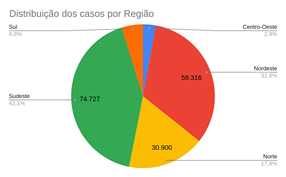
\includegraphics[width=.7\linewidth]{investigacao-professor1}

  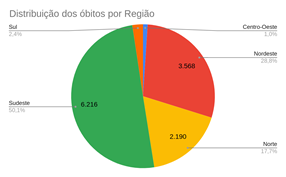
\includegraphics[width=.7\linewidth]{investigacao-professor2}
  \end{figure}

  No entanto, é importante que surja a questão dos dados relativos, e utilizem as demais colunas da tabela. Neste caso, o coeficiente de incidência e de mortalidade da região Norte eram os mais elevados, com 168 casos e 11,9 mortes a cada 100 mil habitantes. Para expressar essa resposta, poderão fazer um gráfico de colunas.

  Uma ideia, para para comparar o número bruto com o relativo é usar gráficos com duas colunas por região, uma indicando o número total de óbitos da região (com marcação da escala no eixo esquerdo) e outro com o coeficiente de mortalidade (com marcação da escala no eixo direito).

  \begin{figure}[H]
  \centering

  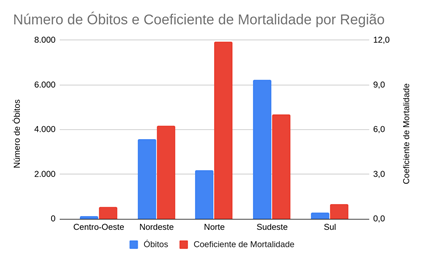
\includegraphics[width=\linewidth]{investigacao-professor3}
  \end{figure}

  Reforça-se a importância de evidenciar que a pergunta não está objetivamente bem formulada e que mesmo estas análises não respondem completamente a questão sobre qual era a região mais afetada, pois como já foi dito, essa ideia não foi conceituada. Para melhorar a análise, é preciso aprofundar-se em outros indicadores, de outras dimensões, montar algum critério quantitativo que capte o sentido de “região mais afetada” e ajude na comparação entre as regiões.

  No item \titem{c)}, é esperado promover uma reflexão sobre as possibilidades que as informações proporcionais podem trazer para uma compreensão mais aprofundada sobre um fenômeno no qual é necessário comparar populações diferentes. A passagem do pensamento aditivo para o proporcional nem sempre é simples para os estudantes e ajudá-los a perceber suas vantagens é importante para que eles se interessem por este outro olhar.

  No item \titem{d)}, o estudante pode apenas comparar duas regiões da tabela, mas espera-se que inicie uma discussão sobre outras formas de afeto. É esperado que nesta questão ele consiga realizar uma comparação um pouco mais complexa, analisando a situação escolhida para a comparação tanto pelo enfoque dos valores absolutos, quanto pelo dos valores proporcionais.  

}{9}
\end{answer}

\begin{task}{Calculando e interpretando dados da COVID-19 por região}

A tabela a seguir apresenta o tamanho da população e os dados brutos do número de casos e de óbitos pela COVID-19 em cada região do Brasil no dia 12 de maio de 2020.

\begin{enumerate}
\item Complete a tabela calculando os coeficientes de indicência, de mortalidade e a taxa de letalidade de cada Estado.
\item Qual região era, até aquele momento, a mais afetada pela COVID-19? Justifique.
\item Você percebeu vantages e desvantagens de se utilizar os coeficientes e taxas? Quais?
\item Como a sua região estava afetada pela COVID-19 naquele momento? Faça a comparação com os dados de outras regiões.
\item Compartilhe suas descobertas com seus colegas.
\end{enumerate}

\begin{table}[H]
\centering
\setlength\tabcolsep{4pt}
\begin{tabu} to \textwidth{|c|r|r|r|r|r|r|}
\hline
\thead
Região & População & Casos & Óbitos & \makecell{Coeficiente de \\ Incidência} & \makecell{Coeficiente de \\ Mortalidade} & \makecell{Taxa de \\ Letalidade} \\
\hline
Centro-Oeste & 16 297 074 & 5 090 & 129 & & & \\
\hline
Nordeste & 57 072 654 & 58 316 & 3 568 & & & \\
\hline
Norte & 18 430 980 & 30 900 & 2 190 & & & \\
\hline
Sudeste & 88 371 433 & 74 727 & 6 216 & & & \\
\hline
Sul & 29 975 984 & 8 556 & 297 & & & \\
\hline
\end{tabu}
\caption{Fonte: \href{https://COVID.saude.gov.br/}{Ministério da Saúde} (Consulta em 12 de Maio de 2020)}
\end{table}
\end{task}

\begin{example}{Outras dimensões da epidemia}
	
Antes da pandemia chegar em terras tupiniquins, acompanhávamos os impactos catastróficos causados em outras regiões do mundo. Receosos, especulávamos sobre como, quando e em que medida ela atingiria nossa nação? Seria também catastrófica ou seria apenas uma gripezinha? Nosso sistema de saúde público conseguiria dar conta? Todos os indivíduos teriam o mesmo acesso ao tratamento? E os impactos em nossa economia? Quais setores produtivos seriam considerados essenciais para nossa sociedade? E aqueles trabalhadores de setores considerados não essenciais, como poderiam garantir o seu sustento? Sobre a estratégia do isolamento social, como colocá-la em prática em locais com grandes aglomerados de pessoas, como nas favelas, nos presídios, etc.? Resumindo, considerando a nossa estrutura social, econômica e cultural, a pergunta geral era: como faríamos para enfrentar a pandemia?

Quando a doença deu seus primeiros sinais por aqui, essas questões começaram a ter respostas concretas. Pesquisadores de várias áreas, sobretudo nas universidades e institutos de pesquisa, trabalhavam arduamente para compreender o seu avanço.

O estudo da Funcação Oswaldo Cruz\footnote{Que pode ser acessado em \url{  https://agencia.fiocruz.br/estudo-aponta-maior-aceleracao-da-COVID-19-no-norte-e-nordeste}}, divulgado em 29 de maio, mostrou que o ritmo de aumento do avanço da covid-19 nas regiões Norte e Nordeste foi muito maior do que no restante do país. O estudo sugeriu a existência de uma relação entre esse aumento e os recursos de cada região.

\begin{quote}
"O Amazonas passou de uma taxa de 493 casos por milhão de habitantes em abril, para 5 300 em maio. O Amapá passou de 492 para 5 100. Roraima, de 366 para 3 266 e Ceará, d3 356 para 3 078. Na comparação, estados com mais recursos parecem menos atingidos pela pandemia, como por exemplo o Paraná, onde a taxa passou de 86 para 217, e o Rio Grande do Sul, de 75 para 329."
\flushleft

(Agência Fiocruz de notícias, 29/05/2020)
\end{quote}

Ou \href{https://drive.google.com/file/d/1tSU7mV4OPnLRFMMY47JIXZgzkklvkydO/view }{estudo}, do Núcleo de Operações e Inteligência em Saúde (NOIS), da PUC-Rio, divulgado no dia 28 demaio, realizou uma análise socioeconômica da taxa de letalidade da COVID-19 no Brasil buscando mostrar que as altas taxas são influenciadas pelas desigualdades no acesso ao tratamento. Para chegas às conclusões, foram cruzadas informações obtidas em duas plataformas públicas: o \href{https://opendatasus.saude.gov.br/}{OpenDataSUS}, que traz dados sobre a saúde no Brasil, e o \href{http://atlasbrasil.org.br}{Atlas de Desenvolvimento Humando do Brasil}, que traz indicadores sociais e econômicos, como o Índice de Desenvolvimento Humano (IDH), o índice de Gini, o Índice de Vulnerabilidade Social, a distribuição da população por classe, gênero e raça, por nível de escolaridade entre outros.

Um dos gráficos apresentados por esse estudo, por exemplo, mostrou a proporção de óbitos ou recuperados por escolaridade e por Raça/Cor.

\begin{figure}[H]
\centering
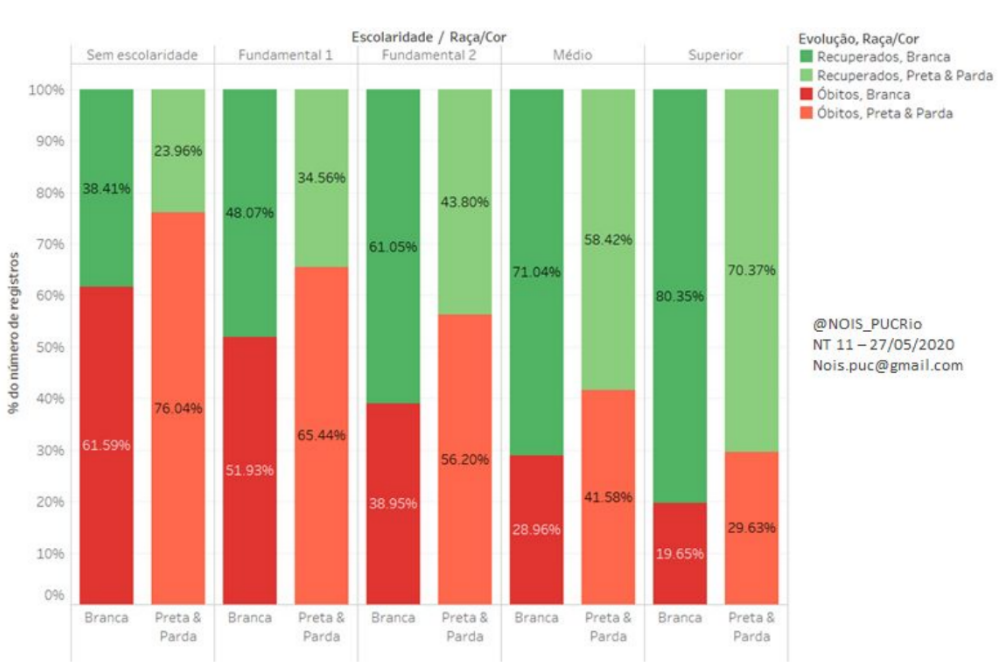
\includegraphics[width=\linewidth]{investigacao2}

\end{figure}

Impactos na economia também começaram a aparecer mais fortemente em indicadores como o Produto Interno Bruto (PIC) e as taxas de ocupação do trabalho. Em 29 de maio, o IBGE divulgou que "o PIB apresentou contração de 1,5\% na comparação do primeiro trimestre de 2020 contra o quarto trimestre de 2019, na série com ajuste sazonal. A Indústria (-1,4\%) e os Serviços (-1,6\%) apresentaram recuo, enquanto a Agropecuária (0,6\%) cresceu"\footnote{\url{https://agenciadenoticias.ibge.gov.br/agencia-sala-de-imprensa/2013-agencia-de-noticias/releases/27837-pib-cai-1-5-no-1-trimestre-de-2020}}. Quanto às taxas de ocupação do trabalho, dados da Pesquisa Nacional por Amostra de Domicílios Contínua (PNAD Contínua), revelaram que "a taxa de desocupação passou de 11,2\% para 12,6\% no trimstre terminado em abril, atingindo 12,8 milhões de desempregados"\footnote{\url{https://agenciadenoticias.ibge.gov.br/agencia-noticias/2012-agencia-de-noticias/noticias/27821-desemprego-atinge-12-6-no-trimestre-ate-abril-com-queda-recorde-na-ocupacao}}.

Como percebemos, os dados nos ajudam a compreender diversas dimensões de uma situação. Tratar de cada uma delas separadamente pode nos dar objetividade, mas certamente é insuficiente para propor soluções amplas. Por isso, podemos dividir tarefas para organizar essas informações, mas é sempre importante trocarmos experiências para compreender a situação de forma mais ampla e não cair em ilusões de soluções simplistas para problemas complexos.
\end{example}


\know{Pirâmide etária}

Não é um indicador na forma de um número, mas sim da distribuição de idades de uma população. A partir dela é possível obter informações sobre natalidade, longevidade e idade média da população.

Do ponto de vista matemático, este indicador é apenas uma contagem de quantas pessoas existem por faixa de idade.

No Brasil este indicador é produzido anualmente pelo IBGE, por meio da Pesquisa Nacional por Amostra de Domicílio Contínua (PNAD Contínua). Na imagem a seguir apresenta uma comparação entre os dados de pirâmide etária do Brasil de 2012 e 2019. Quais informações sobre natalidade, longevidade e idade média da população obter por meio dessa comparação?

\begin{figure}[H]
\centering

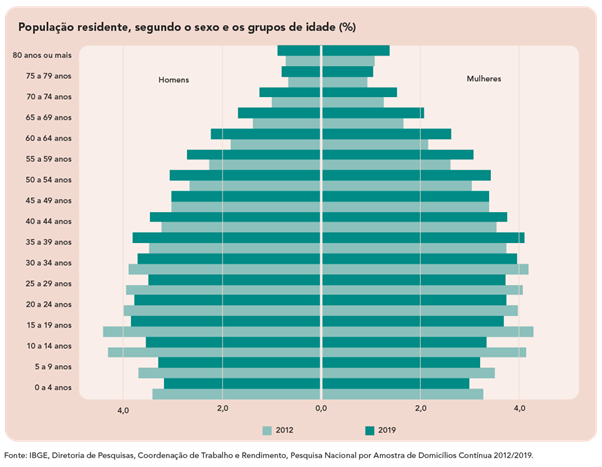
\includegraphics[width=\linewidth]{investigacao7}
\caption{Fonte: \href{https://educa.ibge.gov.br/jovens/conheca-o-brasil/populacao/18318-piramide-etaria.html}{IBGE - PNAD Contínua}}
\label{}
\end{figure}

\know{Índice de atendimento total de esgoto}

Este é um indicador que tenta traduzir em um único número a quantidade de pessoas de um dado município, estado, região ou país atendidas pela rede de esgoto. Ele é calculado por meio de uma razão:


\begin{equation*}
\resizebox{\hsize}{!}{
$
\text{Índice de atendimento total de esgoto}=\frac
{\text{População atendida com esgoto na região de interesse (área rural e urbana)}}
{\text{População total da região de interesse}}
$
}
\end{equation*}


O índice varia entre $0$ e $1$, mas pode ser também apresentado em forma percentual. Quanto mais próximo de $1$ (ou de $100$, no caso da porcentagem), maior é a proporção de pessoas da região de interesse com atendimento de esgoto.

No Brasil o índice é calculado pelo Sistema Nacional de Informação sobre Saneamento (SNIS). Observe o gráfico abaixo produzido com os dados de 2018. A partir dele o que você observa sobre a coleta de esgoto no Brasil?



\begin{figure}[H]
\centering

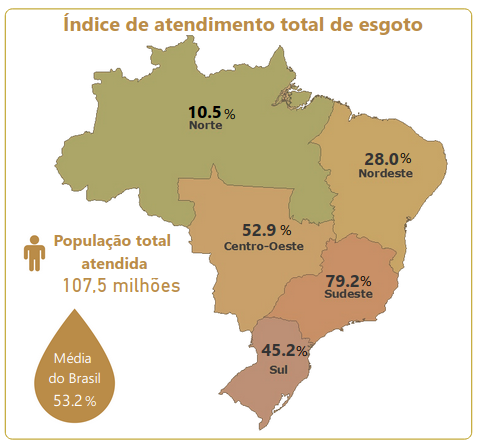
\includegraphics[width=.8\textwidth]{investigacao8}

\caption{Fonte: Ministério do Desenvolvimento Regional - Sistema Nacional de Informação sobre Saneamento. Gráfico obtido do painel de informações sobre saneamento no Brasi \href{http://www.snis.gov.br/painel-informacoes-saneamento-brasil/web/painel-esgotamento-sanitario}{Sistema Nacional de Informação sobre Saneamento. Gráfico obtido do painel de informações sobre saneamento no Brasi}}
\end{figure}

\know{Leitos hospitalares por mil habitantes}

Indicador sobre a quantidade de leitos hospitalares disponíveis pelo sistema público de saúde para a população. Ele pode ser utilizado como uma medida de acesso à saúde. No Brasil, os dados são coletados e disponibilizados pelo Sistema Único de Saúde (SUS), por meio do sistema DataSUS. 

Seu cálculo é dado pela razão
\begin{equation*}
\resizebox{\hsize}{!}{
$
\text{Leitos hospitalares por mil habitantes}=\frac
{\text{Número médio anual de leitos hospitalares conveniados ou contratados pelo SUS}}
{\text{População total residente, ajustada para o meio do ano}}\times1.000
$
}
\end{equation*}

Para saber mais porque a razão é multiplicada por mil, volte e leia a discussão do \hyperref[primeiras-informacoes]{Exemplo 1: Primeiras informações sobre a pandemia}. 

Com este indicador é possível identificando situações de desigualdade entre regiões do país e tendências nas variações geográficas e temporais de leitos hospitalares ofertados pelo SUS. Ele também pode ser usado para subsidiar o planejamento de políticas públicas voltadas para a assistência hospitalar no país.

Na tabela a seguir é possível encontrar os dados temporais de disponibilidades de leitos. Quais desigualdades e tendências você observa?

\begin{figure}[H]
\centering

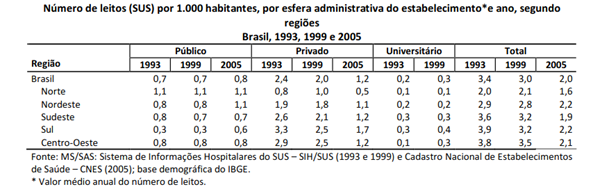
\includegraphics[width=.9\textwidth]{investigacao9}
\end{figure}

\know{Índice de vulnerabilidade social (IVS)}
\clearmargin

\begin{objectives}{}
{
  O objetivo específico desta atividade é ajudar os estudantes a compreenderem a necessidade de analisar os problemas da vida real a partir de várias dimensões e de seus indicadores.
}{1}{0}
\end{objectives}
\begin{sugestions}{}
{
  O texto do exemplo 2 e a atividade pretendem provocar nos estudantes a necessidade de olhar para os problemas da realidade em suas diversas dimensões e indicar alguns caminhos para iniciar uma análise mais aprofundada delas. Em outras palavras, dão subsídio para que o estudante faça suas questões de forma mais fundamentada e objetiva.
}{1}{0}
\end{sugestions}
\begin{answer}{}
{
Algumas respostas esperadas para o item \titem{a)}:

\begin{itemize}[wide]
\item \textbf{Pirâmide Etária}: não é exatamente um indicador na forma de um número, mas sim um indicador da distribuição da população. Há informações de que a Covid é mais letal em idosos. Assim, uma possibilidade de investigação seria verificar a mortalidade por faixa etária, e para isso precisaŕiamos utilizar a pirâmide etária da população estudada.

\item \textbf{Leitos hospitalares por habitante}: Há uma preocupação sobre a possível falta de leitos para atendimentos da doença. Além disso, a distribuição de leitos por habitante não é homogênea. Assim, questões possíveis de serem investigadas dizem respeito a como é o atendimento médico em regiões diversas. Para isso, o número de leitos por habitante é um importante indicador.

\item \textbf{Índice de atendimento total de esgoto}: O atendimento de esgoto é um indicador das condições sociais de uma região, além de estar diretamente relacionado às questões sanitárias. Talvez não seja um indicador tão importante para analisar as questões relacionadas à Covid.

\item \textbf{Índice de Vulnerabilidade Social (IVS)}: Conforme expresso na atividade disparadora, há indicativos de que a Covid tem afetado populações distintas de formas distintas, e que isso teria relação com a condição social. Além disso, esse índice envolve mais de uma dimensão, como o trabalho. Pessoas que exercem trabalhos mais precarizados não conseguem realizar a quarentena de forma efetiva, e portanto estariam mais expostas à contaminação. Outra questão se refere ao acesso ao tratamento, que também é mais precário para pessoas de baixa condição social.
\end{itemize}
}{1}
\end{answer}


Este indicador é formado pela composição de vários outros, é o que se chama de indicador multidimensional. Sua intenção é resumir em um único valor múltiplos parâmetros relacionados ao bem estar de uma população. Estes parâmetros são uma composição de indicadores de três grandes grupos:

\begin{itemize}
\item \textbf{Capital humano}: calculado por meio de uma média simples de 8 indicadores.
\item \textbf{Renda e trabalho}: calculado por meio de uma média simples de 5 indicadores.
\item \textbf{Infraestrutura urbana}: calculado por meio de uma média ponderada de 3 indicadores.
\end{itemize}

Por fim, o IVS é calculado por meio de uma média simples dos três indicadores que o compõe:

\begin{equation*}
\text{IVS}=\frac
{\text{IVS\sub{capital humano}+IVS\sub{renda e trabalho}+IVS\sub{infraestrutura urbana}}}
{3}
\end{equation*}

\begin{table}[H]
\centering

\begin{tabu} to \textwidth{|l|r|r|r|r|}
\hline
\tmcol{5}{|c|}{\parbox[c][1cm][c]{.6\textwidth}{ \centering Índice de Vulnerabilidade Social  Capitais da Região Norte do Brasil - 2010}} \\
\hline
\tmcol{1}{|c|}{Cidade} & \tmcol{1}{c|}{IVS Total} & \tmcol{1}{c|}{\makecell{IVS \\ Infraestrutura urbana}} & \tmcol{1}{c|}{\makecell{IVS Capital\\humano}} & \tmcol{1}{c|}{\makecell{IVS Renda e \\ trabalho}} \\
\tcolor{Rio Branco - AC} & $0{,}339$ & $0{,}276$ & $0{,}433$ & $0{,}307$ \\
\hline
\tcolor{Macapá - AP} & $0{,}339$ & $0{,}271$ & $0{,}433$ & $0{,}307$ \\
\hline
\tcolor{Manaus - AM} & $0{,}387$ & $0{,}458$ & $0{,}388$ & $0{,}314$ \\ 
\hline
\tcolor{Porto Velho - RO} & $0{,}322$ & $0{,}372$ & $0{,}364$ & $0{,}230$ \\
\hline
\tcolor{Boa Vista - RR} & $0{,}261$ & $0{,}157$ & $0{,}362$ & $0{,}265$ \\
\hline
\end{tabu}

\caption{Fonte: Atlas de Vulnerabilidade Social - IPEA}
\end{table}

Para saber quais os indicadores que compõem cada um dos grupos do IVS e seus respectivos pesos, você pode acessar a publicação do IPEA “\href{http://ivs.ipea.gov.br/images/publicacoes/Ivs/publicacao_atlas_ivs.pdf}{Atlas da vulnerabilidade social dos municípios brasileiros}”. Nele, na seção de “conceito e metodologia” você pode encontrar a lista completa dos indicadores que compõem o IVS.

\begin{task}{}

O texto anterior trouxe a ideia de que podemos utilizar informações quantitativas e indicadores para compreender algumas dimensões dos problemas causados pela pandemia.

\begin{enumerate}
\item A seguir apresentamos as definições de alguns indicadores. Escreva como você imagina que cada um deles pode estar relacionado com a pandemia.

\begin{itemize}[itemsep=1em]
\setlength\parskip{-2pt}
\item \textbf{Pirâmide Etária}

\textbf{Descrição}: Quantidade de pessoas de uma região separadas por faixa etárias.

\textbf{Fonte}: IBGE - \href{https://www.ibge.gov.br/estatisticas/sociais/populacao/25089-censo-1991-6.html?=&t=o-que-e}{Censo} e \href{https://www.ibge.gov.br/estatisticas/sociais/populacao/9173-pesquisa-nacional-por-amostra-de-domicilios-continua-trimestral.html?t=destaques}{PNAD Contínua}

\item \textbf{Leitos hospitalares por habitante}

\textbf{Descrição}: Proporção do número de leitos hospitalares por habitante

\textbf{Fontes}: \href{https://datasus.saude.gov.br/}{Ministério da Saúde - DataSUS}; Secretarias de Saúde Estaduais e Municipais

\item \textbf{Índice de atendimento total de esgoto referido aos municípios atendidos com água}

\textbf{Descrição}: Percentual da população atendida por rede coletora de esgoto (com ou sem tratamento) em relação à população total.

\textbf{Fonte}:\href{http://www.snis.gov.br/painel-informacoes-saneamento-brasil/web/painel-setor-saneamento}{Sistema Nacional de Informações sobre Saneamento (SNIS)}


\item \textbf{Índice de Vulnerabilidade Social (IVS)}

\textbf{Descrição}: Indicador que sintetiza informações de infraestrutura, escolaridade e trabalho de grupos populacionais.

\textbf{Fonte}: \href{http://ivs.ipea.gov.br/index.php/pt/}{IPEA} (com dados do censo de IBGE)
\end{itemize}

\item Você conhece outras dimensões dos problemas causados pela pandemia? Que tipos de indicadores você acha que seriam importantes para analisar essas dimensões?

\end{enumerate}


\end{task}

\clearpage
\def\currentcolor{session1}
\begin{paginatexto}{Elaboração de questões - Etapa 2}
{
\textit{(Tempo estimado 2-3 aulas)}

Esta etapa tem como objetivos definir as perguntas de investigação, que orientarão todo o trabalho do capítulo daqui para frente, e os integrantes dos grupos de pesquisa. 

Ela se inicia com a discussão sobre quais devem ser os critérios adotados para formular as perguntas de investigação e utiliza critérios para limitar o universo possível de investigação dos estudantes, de forma a facilitar o trabalho do educador e garantir os objetivos conceituais e metodológicos do capítulo. Desta forma, as perguntas de investigação formuladas pelos estudantes devem ser:

\begin{itemize}
\item \textbf{Quantitativas}

A supressão deste critério traz o risco dos estudantes realizarem perguntas investigativas dentro do tema, mas que são respondidas por meio de análises nas quais a matemática tem pouco ou nenhum papel. Este critério tem a função de manter as investigações dentro dos objetivos pedagógicos e conceituais da disciplina de matemática. 

\item \textbf{Exequíveis} 

Lembre-se que este capítulo é pensado de forma a ser desenvolvido em um mês de atividades (com base em um curso de matemática com 5 aulas de 50 minutos por semana) e que foi pensado com seguinte distribuição de aulas: 
2-3 aulas para a atividade disparadora
2-3 aulas para a elaboração das perguntas de investigação
4-5 aulas para a elaboração do planejamento 
7-8 aulas para o desenvolvimento da investigação
4-5 aulas para a produção do produto final e compartilhamento
Ter mais ou menos tempo para dedicar a cada etapa define a complexidade e profundidade das questões investigativas e das análises que os estudantes podem propor.

\item \textbf{Comparativas}

Questões comparativas limitam o universo possível do estudante investigar. Esse é um critério de simples compreensão e exemplificação para os estudantes e bastante efetivo em limitar a complexidade das análises.
interessantes e/ou sedutoras
O engajamento é fundamental para o desenvolvimento da autonomia e da autorregulação para o estudo. Trabalhar com perguntas investigativas desinteressantes faz com que os estudantes se envolvam menos na proposta.

\item \textbf{Simples}

Este critério tem a função de reforçar a limitação do que é possível investigar no ambiente escolar, garantido que o projeto todo caiba em um período possível no planejamento da disciplina e seja concretizado apesar de possíveis limitações materiais.
\end{itemize}

O livro do estudante traz um exemplo de elaboração de pergunta investigativa, num processo que se inicia com uma questão que não atende os critérios propostos, mas que vai sendo re-elaborada até passar a atender todos eles. Estes critérios devem ser modulados de acordo com a realidade de cada escola. Por exemplo, em uma situação escolar na qual não é possível que os estudantes realizem pesquisas pela internet para coletar dados, é possível olhar para a própria comunidade e fazer a coleta em campo. Neste caso, as perguntas de investigação devem ser limitadas àquelas nas quais os educandos conseguem as informações para montar seus próprios indicadores a partir de entrevistas com a comunidade local.

Ao mesmo tempo que é imprescindível definir critérios para a elaboração de perguntas para investigação no projeto, é igualmente importante possibilitar que os estudantes possam se dedicar a questões de interesse próprio. É a partir deste espaço que os estudantes podem significar sua experiência escolar e de aprendizagem de uma forma mais saudável, significativa e satisfatória. Relatos sobre experiências de aberturas curriculares para os estudantes podem ser encontrados em \citep{singer2010,appleton2017,hecht2016}.
Um cuidado: ter muitos estudantes investigando assuntos diferentes é um grande desafio. Assim, uma possibilidade bem interessante é organizá-los em grupos por tema de interesse. Para isso o educador pode classificar as perguntas investigativas propostas pelos alunos e alunas em diferentes subtemas e juntar os estudantes que propuseram investigações do mesmo subtema. O grupo (que idealmente deve conter por volta de 4 integrantes) deve chegar em uma pergunta única, que será investigada coletivamente.

É interessante utilizar uma ficha para que os estudantes pratiquem a elaboração de perguntas investigativas que atendam todos os critérios. Estas fichas com as questões iniciais de cada estudante e a questão definida pelo grupo podem ser arquivadas conjuntamente, de forma a construir um portfólio do percurso dos estudantes e do grupo, ao ser alimentado com novos materiais a cada etapa da pesquisa. Um exemplo de ficha está ao \hyperref[elaboracao-questoes]{final do capítulo}

}
\end{paginatexto}

\explore{Elaboração de Questões - etapa 2}
\phantomsection\label{etapa2}
\phantomsection\label{pergunta-cientifica}
\vspace{-.5\baselineskip}
\subsection{O que é uma boa pergunta científica?}

Nós, seres humanos, podemos ser muito diferentes uns dos outros. No entanto, existe algo que nos unifica: absolutamente, todos nós temos problemas. Decerto, eles podem variar muito. Algumas pessoas precisam se preocupar constantemente com o trabalho que precisam executar para conseguir alguma remuneração para comprar produtos que consideram necessários a sua sobrevivência. Outras passam longe desse tipo de preocupação, mas muitas vezes não encontram sentido profundo em suas vidas, deprimindo-se.

Em ambos os casos, não há escapatória: se não podemos solucionar esses problemas seremos soterrados por eles. Portanto, nosso cotidiano é uma dimensão da vida na qual precisamos constantemente dar respostas aos nossos problemas. De preferência, rapidamente, para que não se acumulem e nos prejudiquem.

Deste modo, a qualidade das nossas respostas interfere diretamente em nosso cotidiano. E conseguimos dar respostas melhores quando conseguimos entender melhor nossos problemas, quando conseguimos elaborá-los na forma de perguntas. Em outras palavras, conseguimos expressar nossa humanidade de maneira mais vívida quando somos curiosos.  

Mas a velocidade exigida pelo cotidiano dificulta a formulação das perguntas. A necessidade de respostas rápidas desorienta nossos esforços em busca de exercitar nossa curiosidade. É por isso que outra dimensão da vida é imprescindível: a ciência.

Independentemente da área do conhecimento, o desenvolvimento científico é todo baseada em perguntas. Quando querem investigar algum processo, fenômeno ou aparato, os cientistas elaboram uma pergunta relacionada ao seu objeto/tema de estudo e se concentram nela. 

A investigação desenvolvida neste capítulo tem limitações se comparada ao trabalho dos cientistas. Uma delas é a questão do tempo, dado que o tempo da escola é muito diferente do tempo do universo acadêmico. Assim, neste projeto não é possível realizar questionamentos muito complexos e investigações realmente aprofundadas. Para adequar a proposta ao tempo e objetivos da escola, as perguntas científicas trabalhadas aqui precisam seguir certos critérios:

\begin{itemize}
\item elas devem ser quantitativas, ist é, devem estar relacionadas a quantidades e/ou informações numéricas;
\item precisam ser exequíveis num período de tempo apropriado (e por isso não podem demandar anárlises muito longas ou complexas);
\item é necessário que sejam comparativas, ou seja, avaliar diferentes situações ou a mesma situação em localidades diferentes, etc;
\item busquem ser interessantes, de forma que não sejam respondidas com uma simples busca na internet;
\item e sjeam simples, restritas a situações pouco complexas ou olhar para apenas um fator de uma determinada situação.
\end{itemize}


% \begin{table}[H]

% \centering
% \begin{tabu} to \textwidth{|c|>{\vspace{3pt}}m{.3\textwidth}<{\vspace{3pt}}|m{.3\textwidth}|}
% \hline
% \thead
% Característica & Adequada & Inadequada \\
% \hline
% \cellcolor{white}\textcolor{black}{\textbf{Quantitativa}} & O índice de pessoas afetadas pela Covid em minha escola é maior ou menor do que na minha cidade? & Como se sentiram as pessoas infectadas em minha escola?\\
% \hline
% \cellcolor{white}\textcolor{black}{\textbf{\makecell{Exequível em \\ tempo apropriado}}} & Qual a taxa de ocupação das famílias de minha turma antes e depois da pandemia? & Qual a taxa de pessoas ocupadas em minha região antes e depois da pandemia? \\
% \hline
% \cellcolor{white}\textcolor{black}{\textbf{Comparativa}} & A taxa de letalidade da Covid é a mesma nas comunidades indígenas e nos grandes centros urbanos brasileiros? & A taxa de letalidade da Covid é a mesma para diferentes populações do Brasil?\\
% \hline
% \cellcolor{white}\textcolor{black}{\textbf{Sedutora/interessante}} & Qual foi o impacto da quarentena em minha região na contenção da pantemia? & Quam não tem acesso à rede de água e esgoto foi mais afetado pela Covid? \\
% \hline
% \cellcolor{white}\textcolor{black}{\textbf{Simples}} & Qual região da minha cidade apresentou a maior taxa de disseminação da Covid? & Qual a taxa de disseminação da Covid em minha turma? \\
% \hline
% \end{tabu}
% \end{table}

% Vejam que as perguntas da segunda coluna apresentam características que, embora não as tornem desnecessárias para a compreensão da realidade, as tornam inviáveis no contexto da sala de aula. Elas não permitem um aprofundamento metódico nos estudos matemáticos se estiverem orientadas a tentar compreender a subjetividade dos sujeitos envolvidos. Tampouco pode ser objetiva e, ao mesmo tempo, extremamtente abrangente, inviabilizando sua feitura nos prazos possíveis. O mesmo ponto sobre a abrangência vale para os casos de comparação possíveis: quanto mais genérica a comparação, mais difícil será efetivá-la. E, por fim, as perguntas não podem querer validar sua opinião, seja na confirmação de uma opinião amplamente aceita, seja na limitação rasteira do seu objeto.

% Você não precisa se preocupar em tentar solucionar os grandes problemas do mundo. Pelo menos não por agora. Afinal, estas grandes questões demandam um esforço que foge aos limites da pesquisa em sala de aula.

% Mas isso não significa que você deva abandonar esse desejo. Ao contrário, nossa intenção é que você seja cada vez mais capaz de alcançar essa possibilidade. Para isso, cabe um exercídio: dividir essa pergunta comiplexa em perguntas mais simples. Ao serem satisfatoriamente respondidas, nos enriquecem do conhecimento necessário para tratar de questões mais complexas, nos fazendo galgar degraus até nosso interesse final.

\begin{task}{Elaboração de boas perguntas científicas}

Elabore três perguntas investigadas sobre as pectos do seu tema. Tente seguir os critério mencionados anteriormente. Utilize as atividades do "\hyperref[primeiras-informacoes]{Explorando: Primeiras Informações Sobre a Pandemia}"{} como inspiração. Ao fazer as atividades e ler o texto daquela seção, quais curiosidades e questionamentos vieram à sua mente?

Uma dica: Ao pensar em perguntas tente imaginar como você faria para respondê-las. Que tipo de dados, medidas ou observações seriam necessárias? Se você não souber por onde começar, provavelmente você pensou em uma pergunta é complexa

Depois de verificar com sua professora ou seu professor se as três questões formuladas atendem todas as características para se enquadrarem como uma boa pergunta, será hora de se juntar com colegas que tenham interesse por recortes temáticos parecidos com o seu e definir qual será a pergunta de investigação de seu grupo.

Escreva em seu caderno a pergunta na qual você irá se aprofundar. Lembre-se que ela tem que atender a todas as características discutidas no texto "\hyperref[pergunta-cientifica]{O que é uma boa pergunta científica}".

\end{task}

\begin{task}{elaboração de questões do projeto sobre COVID-19}

Veja o diálogo entre o estudante Rodrigo e a sua professora.

\begin{quote}
\textbf{Rodrigo}: Professora, estive pensando em investigar como a pandemia afetou os nossos empregos.

\textbf{Professora}: Este me parece um questionamento interessante, Rodrigo. Mas vejamos se ele atende nossos critérios. Em primeiro lugar, como expressar esse problema de forma quantitativa?

\textbf{Rodrigo}: Não sei exatamente, professora.

\textbf{Professora}: Bem, penso que precisamos de indicadores de emprego. Você conhece algum?

\textbf{Rodrigo}: Eu vi matérias nos jornais dizendo que o desemprego estava alto. Falaram que $13\%$ das pessoas estavam desempregadas.

\textbf{Professora}: Exatamente, a taxa de desemprego é um indicador, que no Brasil é calculado pelo IBGE. É possível também olhar para a taxa de pessoas ocupadas, que são aquelas exercem algum trabalho. O que você prefere olhar? Como podemos então formular a pergunta?

\textbf{Rodrigo}: Acho que prefiro olhar para as pessoas ocupadas. A pergunta poderia então ser: “qual é a taxa de pessoas ocupadas durante a pandemia?”

\textbf{Professora}: De quais pessoas você está falando?

\textbf{Rodrigo}: Pensei em investigar entre os colegas de turma. Talvez perguntar sobre os familiares da minha classe. 

\textbf{Professora}: Legal. Você já tem uma pergunta que é simples, quantitativa e que me parece ser possível de respondermos em um tempo adequado. Mas ela não é comparativa, e também não responde à questão de como os empregos foram afetados pela pandemia.

\textbf{Rodrigo}: Podemos perguntar quais eram as taxas de ocupação dos familiares de minha classe antes da pandemia e compará-la com as atuais?
Professora: Creio que estamos num bom caminho. Tente formular a pergunta de forma objetiva.

\textbf{Rodrigo}: Qual era a taxa de ocupação dos familiares da minha classe antes da pandemia e qual é a taxa atual? Que tal?

\textbf{Professora}: Para deixar sua pergunta mais interessante, que acha de comparar essas taxas com as do país? Assim você teria uma ideia da relação entre a nossa turma e a realidade nacional.

\textbf{Rodrigo}: Gosto da ideia! Então ficaria assim: Qual era a taxa de ocupação dos familiares da minha classe antes da pandemia e qual é a taxa atual? E como essas taxas se comparam com as nacionais?

\end{quote}

Repare no diálogo entre Rodrigo e sua professora, apresentado no exemplo logo acima. Perceba que ele começou elaborando uma pergunta que não se encaixava em todos os critérios necessários para o projeto, mas que com ajuda foi reformulando a questão até ter algo que atendia a todos os critérios estabelecidos para o projeto.

As questões elaboradas pelo Rodrigo nesse processo, embora não sejam desnecessárias para a compreensão da realidade, são inviáveis no contexto de sala de aula. Elas não permitem um aprofundamento metódico nos estudos matemáticos se estiverem orientadas a tentar compreender a subjetividade dos sujeitos envolvidos. Tampouco pode ser objetiva e, ao mesmo tempo, extremamente abrangente, inviabilizando sua feitura nos prazos possíveis. O mesmo ponto sobre a abrangência vale para os casos de comparação possíveis: quanto mais genérica a comparação, mais difícil será efetivá-la. E, por fim, as perguntas elaboradas para o projeto não podem querer validar sua opinião, seja na confirmação de uma opinião amplamente aceita, seja na limitação rasteira do seu objeto.

Você não precisa se preocupar em tentar solucionar os grandes problemas do mundo. Pelo menos não por agora. Afinal, estas grandes questões demandam um esforço que foge aos limites da pesquisa em sala de aula.

Isso não significa que você deva abandonar esse desejo. Ao contrário, nossa intenção é que você seja cada vez mais capaz de alcançar essa possibilidade. Para isso, cabe um exercício: dividir essa pergunta complexa em perguntas mais simples.

\end{task}

\clearpage
\begin{paginatexto}{Planejando a Investigação - Etapa 3}
\textit{(Tempo estimado 3-4 aulas)}

\subsection{Introdução}
Ao desenvolver projetos abertos, dois grandes desafios são garantir os objetivos pedagógicos traçados pelo educador e que o projeto tenha início, meio e fim dentro do tempo proposto no cronograma. Neste sentido, o planejamento de como a investigação será executada é um importante aliado, pois permite direcionar o olhar e o trabalho dos estudantes sem obrigar todos a seguirem um mesmo caminho.

Por outro lado, os estudantes do Ensino Médio precisam ainda de orientação para desenvolver um planejamento que seja completo e exequível.
Desta forma, o objetivo específico desta seção é orientar os estudantes em como realizar um bom planejamento de pesquisa. Isso passa por aprofundar a compreensão sobre indicadores, de forma a conseguir avaliar quais são adequados para responder sua pergunta investigativa e como encontrar fontes confiáveis de informações. Os estudantes também devem compreender o conceito de hipótese e relembrar como gráficos diversos, diagramas e tabelas podem ser utilizados adequadamente para evidenciar informações quantitativas.

Nesta etapa do projeto, que se inicia assim que os grupos estão montados, as perguntas têm papel fundamental: 

\begin{enumerate}
\item os grupos devem ter a sua pergunta de investigação definida e 
 
\item as perguntas orientadoras, sugeridas na “Atividade: Roteiro de planejamento da investigação” desta seção, devem ser apresentadas. Entretanto ainda não deve haver a expectativa de responder a todas.
 \end{enumerate} 

Caso haja oportunidade, é interessante entregar uma ficha por grupo com todas as questões que devem ser respondidas no planejamento. Compreender as questões apresentadas nesta ficha de planejamento deve ser a primeira etapa deste processo. Ao formularem uma pergunta, é pouco provável que os estudantes já tenham um plano de como trabalhar para respondê-la. 
É sugerido que após entregar o roteiro de planejamento aos estudantes, eles tenham um tempo (em seus grupos) para discutirem o que acham que já conseguem responder e quais questões necessitam de novas informações/aprofundamentos. O educador pode ir caminhando com os grupos todos meio juntos, fazendo pausas para discussões mais curtas ou mais longas (dependendo das demandas) de forma a irem preenchendo o planejamento ao longo das 3 ou 4 aulas reservadas para esta etapa do projeto.

Uma outra vantagem de utilizar a ficha de planejamento, com todas as questões, é que ela pode ser utilizada como uma ferramenta avaliativa. Pois, ao finalizar a pesquisa é possível verificar os passos propostos, se eles foram seguidos, se as hipóteses foram discutidas na conclusão, etc. 

A questão 1 do roteiro de planejamento dá espaço para a discussão sobre o conceito de hipótese, fundamental no modo de fazer da ciência. Já as questões 2 e 3 do mesmo roteiro, que são sobre os indicadores e perguntam sobre a relação destes com o tema do grupo, são um ótimo momento para fazer uma pausa no projeto e garantir que todos entendam a função dos indicadores e taxas para a compreensão mais aprofundada de um tema. Da mesma forma, a questão 4 traz a possibilidade de realizar uma discussão sobre fontes confiáveis de informações. E as questões 5 e 6 do roteiro abrem oportunidade para retomar estratégias para organizar os dados em gráficos e tabelas, relembrando os tipos de gráficos mais utilizados e seus principais usos. Cabe ao educador, em sala de aula, entender a necessidade de seus estudantes e planejar quais questões do roteiro necessitam de discussões longas e aprofundadas sobre determinados conteúdos e quais demandam discussão curta (apenas para relembrar algumas informações) ou ainda intervenções em grupos pontuais para sanar questões que eventualmente apareçam.

\end{paginatexto}

\def\currentcolor{session4}


\begin{objectives}{Hipóteses}
{
Conceituar hipótese e ajudar os estudantes a identificarem suas hipóteses sobre sua pergunta de investigação. Este é um passo importante que guiará quais dados devem ser coletados e quais análises devem ser feitas, pois o trabalho de investigação tem como finalidade tentar verificar a hipótese inicial e portanto é imprescindível que as hipóteses dos estudantes sejam verificáveis. 

Por exemplo, para responder a hipótese de como o emprego foi influenciado pela pandemia, é necessário definir qual será o grupo alvo do estudo e realizar uma busca por indicadores desse grupo ou, no caso proposto, realizar uma enquete com o alvo. É possível fazer uma discussão sobre quais grupos são mais adequados para a comparação. A hipótese que se quer verificar guia toda a investigação!
}{1}{1}
\end{objectives}



\arrange{Planejando a investigação - etapa 3}
\phantomsection\label{etapa3}

\begin{task}{Roteiro de planejamento da investigação}

A seguir você encontrará algumas perguntas orientadoras para a formulação do planejamento. Em conjunto com seu grupo, você deve responder cada uma das questões, registrando suas respostas em uma ficha ou no caderno. 

\begin{enumerate}[label=\titem{\arabic*)}]
\item Escreva as hipóteses que o você e seu grupo tem sobre a pergunta que escolheram para investigar.

\item A partir de notícias e outras fontes de informação sobre o tema de sua pergunta investigativa façam uma pesquisa e registrem quais são os principais indicadores deste tema.

\item Quais dados vocês usaram para responder a pergunta proposta? Justifiquem explicando a relação entre os dados escolhidos por vocês e a relação deles com a pergunta investigativa do grupo.

\item Quais são as fontes de dados confiáveis para os dados escolhidos por vocês?

\item Expliquem como vocês utilizarão os dados para responder a pergunta investigativa do grupo. Dêem exemplos. Que cálculos vocês farão com esses dados e o que esperam obter? Não se esqueçam que ao final, a análise deve servir para testar a(s) sua hipótese(s) inicial(is).

\item Façam um esboço do(s) tipo(s) de gráfico(s) que vocês utilizarão para apresentar seus dados. Abusem das cores e criatividade em seu esboço. Não se esqueçam de identificar quais dados vocês esperam apresentar em cada gráfico que fizerem. 
\end{enumerate}
\end{task}

\subsection{Hipóteses}

Depois de elaborada a pergunta, é hora de pensar em como respondê-la. É provável que você, ao formular sua pergunta já tenha um palpite do que pode ser a resposta. Ele pode parecer bastante coerente na sua mente, mas é possível que você não consiga expressá-lo em palavras com a mesma desenvoltura. Trata-se mais de intuição do que de raciocínio.

Considerando que a ciência é uma atividade que trabalha com explicações baseadas em evidências, é necessário testarmos nossas ideias intuitivas por meio de observações ou tomadas e análises de dados. Um projeto científico possui esta finalidade: confrontar o pensamento intuitivo com a realidade, demonstrando o alcance de uma certa resposta ao problema colocado a partir de um conjunto de etapas passíveis de serem reproduzidas (verificadas).

A primeira etapa de uma investigação é entender o que você imagina  como resposta para sua pergunta, ou seja, materializar sua intuição em linguagem conceitual, formular aquilo que chamamos de hipótese. Observe o exemplo a seguir, no qual é apresentada uma hipótese para o projeto fictício sobre a COVID-19.


\begin{example}{Planejamento da investigação - COVID-19}

Depois da elaboração das perguntas, a Priscila e o Thiago se juntaram ao Rodrigo para investigar a questão proposta sobre as taxas de ocupação antes e depois da pandemia. Veja o diálogo entre eles:

\begin{quote}
\textbf{Rodrigo}: Olá pessoal, lembro que nossa questão diz respeito às taxas de ocupação dos familiares de nossa classe antes e depois da pandemia, bem como compará-las com as taxas nacionais. Quais são, neste caso, as nossas hipóteses?

\textbf{Thiago}: Bom, eu acho que não mudou muito. Os meus pais continuam trabalhando normalmente.

\textbf{Priscila}: Na minha família teve muita gente que não está conseguindo trabalhar. Meu pai mesmo é vendedor e não pode sair, pois é do grupo de risco. E minha mãe teve que abandonar o emprego pois precisa cuidar da minha irmã pequena em casa.

\textbf{Rodrigo}: Em casa também não mudou muito, mas direto a televisão mostra notícias sobre o aumento do desemprego. Então eu acho que deve ter mudado sim.

\textbf{Thiago}: É, talvez tenha mudado para a maioria. Acho que essa é nossa hipótese.

\textbf{Priscila}: Isso! A nossa hipótese é que muita gente perdeu o emprego. E no Brasil vai ser igual a escola, né?
\end{quote}

\end{example}

\clearmargin
\begin{objectives}{Indicadores da força de trabalho}
{
  O objetivo desta atividade é mostrar ao estudante que os indicadores, apesar de ter uma matemática simples na maioria das vezes, é permeado de escolhas para representar questões específicas. Os quatro primeiros itens da atividade pedem para que os estudantes criem formas de cálculo para expressar a taxa de desemprego e a taxa de subutilização da força de trabalho. Já no item (e) o estudante deve pesquisar a metodologia utilizada pelo IBGE e comparar com a discussão que ele próprio fez.
}{1}{1}
\end{objectives}
\begin{sugestions}{Indicadores da força de trabalho}
{
  A seguir apresentamos as taxas que o IBGE calcula para que vocês, professores, tenham um conhecimento antecipado delas. Vocês verão que ao longo da discussão com os estudantes, eles mesmos irão propor o cálculo igual a uma ou outra taxa já estipulada pelo IBGE.

  Segundo os relatórios da PNAD contínua do IBGE \cite{brasil2020}, são consideradas as seguintes taxas.

  \begin{table}[H]
  \centering
  
  \begin{tabu} to \textwidth{|d{.4\linewidth}|d{.5\linewidth}|}
  \hline
  \tmcol{1}{|c|}{Nome da Taxa} & \tmcol{1}{c|}{Cálculo} \\
  \hline
  Taxa de desocupação & \parbox{\linewidth}{Numerador: Desocupados \\ Denominador: Força de Trabalho} \\
  \hline
  Taxa combinada da desocupação e subocupação & \parbox{\linewidth}{Numerador: Subocupados + desocupados \\ Denominador: Força de trabalho} \\
  \hline
  Taxa combinada da desocupação da força de trabalho potencial & \parbox{\linewidth}{Numerador: Desocupados + Força de Trabalho Potencial  \\ Denominador: Força de Trabalho ampliada} \\
  \hline
  Taxa composta da subutilização da força de trabalho & \parbox{\linewidth}{Numerador: Subocupados + desocupados + força de trabalho potencial \\ Denominador: Força de Trabalho ampliada} \\
  \hline
  Taxa de desalento na força de trabalho ampliada & \parbox{\linewidth}{Numerador: Pessoas deslanetadas \\ Denominador: Força de Trabalho ampliada} \\
  \hline
  Percentual de desalentados na população fora da força de trabalho & \parbox{\linewidth}{Numerador: Pessoas desalentadas \\ Denominador: População fora da Força de Trabalho} \\
  \hline
  Percentual de desalentados na força de trabalho potencial & \parbox{\linewidth}{Numerador: Pessoas desalentadas \\ Denominador: Força de Trabalho potencial} \\
  \hline
  \end{tabu}
  \end{table}

  Professor, perceba as diferentes razões utilizadas pelo IBGE para calcular indicadores das características da força de trabalho. Quais delas deve ser utilizada para indicar o desemprego: a “taxa de desocupação”, ou a “taxa combinada da desocupação e da força de trabalho potencial”, ou alguma outra? Observe que a resposta depende dos objetivos. Se queremos a medida de desemprego apenas entre aqueles disponíveis para trabalhar, calculamos a “taxa de desocupação”. Se, por outro lado, consideramos as pessoas da força de trabalho potencial como desempregadas, calculamos a “taxa combinada”. Por outro lado ainda, poderíamos pensar em fragmentar a força de trabalho ampliada entre aqueles disponíveis para trabalhar e aqueles indisponíveis, considerando apenas os primeiros como desempregados, mesmo que não tenham buscado um emprego. Esperamos que com isso o professor possa encaminhar as discussões com os estudantes.

  Uma discussão análoga deve acontecer propor medida de subutilização da força de trabalho.

}{0}{9}
\end{sugestions}

\begin{answer}{Indicadores da força de trabalho}
{
  A seguir, indicamos algumas possibilidades que devem surgir das respostas dos estudantes.

  No item \titem{a)} é provável que a maioria dos estudantes calcule a taxa de desemprego através da razão entre o número de pessoas ocupadas e o número de pessoas na força de trabalho (é o que o IBGE chama de “taxa de desocupação”). Se feita desta forma, no exemplo dado chegamos a uma taxa de $\dfrac{12.791}{96.138}=13,3\%$. Por outro lado, é possível que se considere como desempregadas as pessoas na força de trabalho potencial. Assim, deveríamos calcular a razão entre a soma do total de desocupados ($12.791$), com o total de pessoas na força de trabalho potencial ($13.542$), e o total de pessoas na força de trabalho ampliada, que é formada pelas pessoas na força de trabalho e mais as pessoas na força de trabalho potencial (é o que o IBGE chama de taxa combinada da desocupação e da força de trabalho potencial). Assim chegamos na taxa de $\dfrac{12.791+13.542}{96.138+13.542}=24\%$. A questão, no final das contas, é compreender o significado da taxa e qual a sua utilidade. Por exemplo, se buscamos compreender o desemprego apenas entre

  No item \titem{b)} também devem aparecer formas distintas de se calcular a taxa. Uma das possibilidades seria calcular a proporção de subocupados dentre os ocupados. Neste caso temos uma taxa de $\dfrac{5.613}{83.347}=6,7\%$. Este cálculo pode ser feito se estamos interessado em compreender apenas quanto dos trabalhadores com alguma ocupação estão trabalhando menos do que poderiam. No entanto, calculada desta forma a taxa não expressa a subutilização mais ampla, pois não inclui os desocupados. Para incluí-los, poderíamos calcular a proporção de subocupados ou desocupados dentro da força de trabalho (é o que o IBGE chama de Taxa combinada da desocupação e subocupação). Neste caso chegamos a uma taxa de $\dfrac{5.613+12.791}{96.138}=19,1\%$. Novamente, esta taxa não considera como subutilizados os trabalhadores na força de trabalho potencial. No entanto, se entendemos que a força de trabalho potencial também é medida de subutilização, poderíamos calcular a razão entre a soma subocupados + desocupados + força de trabalho potencial e a força de trabalho ampliada (é o que o IBGE chama de taxa composta de subutilização). Neste caso chegamos na taxa $\dfrac{5.613+12.791+13.542}{109.680}=29,1\%$.

  Na discussão do item \titem{c)} é necessário ficar atento ao fato de que propostas diferentes de cálculo indicam coisas diferentes. O mais importante aqui é se o método de cálculo corresponde ao fenômeno indicado.

  No item \titem{d)} o professor pode apresentar as taxas calculadas pelo IBGE aos estudantes. Outra recomendação é buscar notícias em jornais e na internet e ver como elas se referem às taxas. Você pode propor uma discussão com os estudantes sobre a matéria, procurando perceber se a forma como se referem às taxas estão condizentes com o que elas realmente querem indicar. Uma sugestão de matéria é \cite{camargo2020}. 

}{0}
\end{answer}
\subsection{Uso de indicadores}

As explicações que construímos sobre a realidade passam pelas ações de identificar e comparar. Percebemos a existência de diferenças e, em seguida, buscamos um jeito de compará-las, usando essas informações para então construir nossas explicações. Uma forma de fazer isso é através da utilização de indicadores. 


Um indicador é um recurso metodológico. Para nossos propósitos, nos interessa que ele seja empiricamente aferido, quantitativo, e que sintetize informações sobre aspectos da realidade ou sobre suas transformações. Um indicador com essas características procura dar objetividade a um conceito que pode ser, a princípio, abstrato.


Podemos representar sua construção em basicamente três etapas:

\begin{enumerate}[label=\titem{\arabic* -}]
\item percepção de eventos empíricos da realidade;
\item obtenção de dados brutos e estatísticas sobre o evento;
\item sintetização dos dados procurando dar-lhes um valor informacional sobre certos contextos.
\end{enumerate}

\begin{figure}[H]
\centering

\begin{tikzpicture}[every node/.style={scale=.9}]
\tikzstyle{quad}=[draw, rectangle, node distance=6cm, align=center, minimum height=2.5cm, minimum width=4cm, fill=\tikzcolor, font=\bfseries, text=white];

\node (a) [quad] {Eventos \\ empíricos \\ da realidade};
\node (b) [quad, right of=a] {Obtenção \\ de dados \\ brutos e \\ estatísticas};
\node (c) [quad, right of=b] {Sintetização e \\ agregação de valor \\ informacional para \\ analisar contextos};

\path[->,very thick]
(a) edge (b)
(b) edge (c);
\end{tikzpicture}

\end{figure}

Apesar da busca de objetividade, não podemos esquecer que a construção de qualquer indicador é realizada por grupos de indivíduos influenciados histórica e socialmente, e que portanto colocam nesses indicadores determinadas visões de mundo. Desta forma, um indicador pode ser objetivo, mas jamais é neutro ou imparcial.

Na maior parte das vezes, a matemática envolvida nos indicadores é bastante simples, se baseando conteúdos como razões, proporções, percentuais, médias, etc. Uma das partes mais difíceis é elaborar categorias e instrumentos de pesquisa que consigam dar conta de expressar a parte da realidade desejada.

A atividade a seguir busca mostrar como esse processo é complicado mesmo com questões aparentemente simples, como encontrar um indicador de subutilização da força de trabalho.

\begin{task}{indicadores da força de trabalho}
A ideia aqui é construir um indicador de quanta força de trabalho está sendo desperdiçada. Uma das possibilidades é simplesmente calcular, dentro da população, quantas estão desempregadas. No entanto, calcular isso desta forma seria muito simples e não captaria outras condições relacionadas à ocupação, como a questão dos indivíduos poderem ou não trabalhar, ou de estarem trabalhando menos do que poderiam, ou ainda sobre as ações tomadas pelos indivíduos na tentativa de realizar algum trabalho. Para dar conta de algumas dessas questões, o IBGE elabora a seguinte divisão das pessoas em idade de trabalhar:

\begin{figure}[H]
\centering

\begin{tikzpicture}[
level/.style={sibling distance = 5.5cm/#1,
level distance = 2cm, scale=1.25}, 
every node/.style={draw, rectangle, minimum width=3cm, minimum height=2cm, node distance=1., label distance=-.45cm, fill=\tikzcolor, text=white, font=\bfseries\small,},
align=center, rounded corners
				   ] 

\node (a) {Pessoas em idade \\de trabalhar \\(14 anos ou\\ mais de idade)}
	child {node [yshift=2cm]{Pessoas na \\ força de \\ trabalho}
			child {node [xshift=2.5cm]  {Pessoas \\ ocupadas}
					}
			child {node [yshift=-2.5cm]  {Subocupadas \\ por insuficiência \\ de horas \\ trabalhadas}
					}
			child {node [xshift=-2.5cm] {Pessoas \\ desocupadas}
					}
			}
	child {node  [yshift=2cm] {Pessoas fora \\ da força \\ de Trabalho}
			child {node [xshift=2.5cm] {Pessoas na\\  força de \\ trabalho \\ não potencial}
					}
			child {node [yshift=-2.5cm]{Pessoas na \\ força de \\ trabalho \\ potencial}
					}
			child {node [xshift=-2.5cm] {Pessoas \\ desalentadas}
					}
			}						
;
\end{tikzpicture}
\end{figure}
\end{task}

Em outras palavras, o IBGE divide as pessoas com 14 anos ou mais de idade em pessoas “na força de trabalho”{} e “fora da força de trabalho”. Dentro da força de trabalho, considera as categorias “ocupadas”{} e “desocupadas”. Dentro das ocupadas, considera ainda as “subocupadas”. Dentre as que estão fora da força de trabalho, o IBGE considera aquelas que formam uma “força de trabalho potencial”. E dentro dessa categoria, considera ainda as “pessoas desalentadas”.
\clearpage
A seguir colocamos algumas breves descrições de cada categoria:

\begin{table}[H]
\centering
\begin{tabu} to \textwidth{|>{\centering}m{.2\textwidth}|>{\vspace{2.5pt}}m{.6\textwidth}<{\vspace{2.5pt}}|}
\hline
\tcolor{Categoria} & \tmcol{1}{|c|}{Descrição} \\
\hline
Força de Trabalho & Pessoas disponíveis para trabalhar. \\
\hline
Ocupadas & Pessoas que exercem algum tipo de trabalho. \\
\hline
Desocupadas & Pessoas que não estão exercendo trabalho e que estão efetivamente em busca de conseguir um emprego. \\
\hline
Subocupadas & Pessoas que trabalham menos de 40 horas na semana e que estão dispostas a trabalhar mais. \\
\hline
Força de Trabalho Potencial & Pessoas que buscaram emprego mas que não podiam assumir no período considerado, ou pessoas que estavam disponíveis para trabalhar mas que não realizaram buscas por emprego. \\
\hline
Desalentadas & Pessoas desempregadas que gostariam de trabalhar, mas que não buscaram emprego pois não tinham esperanças de conseguir. \\
\hline
Força de Trabalho Ampliada & É a soma das pessoas na força de trabalho com as pessoas na força de trabalho potencial. \\
\hline
\end{tabu}
\end{table}

A tabela a seguir mostra os dados brutos da PNAD contínua do segundo trimestre de 2020 referente à essas categorias.

\begin{table}[H]
\centering

\begin{tabu} to \textwidth{|l|c|}
\hline
\tmcol{1}{|c|}{Categoria} & \tcolor{\makecell{Total\\(em milhares de pessoas)}} \\
\hline
Pessoas em idade de trabalhar & 173.918 \\
\hline
Força de Trabalho & 96.138 \\
\hline
Fora da Força de Trabalho & 77.781 \\
\hline
Ocupadas & 83.347 \\
\hline
Desocupadas & 12.791 \\
\hline
Subocupadas & 5.613 \\
\hline
Força de Trabalho Potencial & 13.542 \\
\hline
Desalentadas & 5.683 \\
\hline
Força de Trabalho Ampliada & 109.680 \\
\hline
\end{tabu}
\end{table}

\begin{enumerate}
\item Considerando as categorias e dados acima, qual cálculo você faria para representar a taxa de desemprego? Justifique.
\item Considerando as categorias e dados acima, qual cálculo você faria para representar a taxa de subutilização da força de trabalho? Justifique.
\item Discuta com seus colegas os cálculos que você propôs.
\item Consulte as taxas calculadas pelo IBGE e compare-os com os que foram criados por você e por seus colegas.
\end{enumerate}

\clearpage\begin{objectives}{Fontes confiáveis}
{
  O objetivo desta subseção do Organizando é apresentar aos estudantes formas de busca e identificação de fontes de dados de pesquisa confiáveis. É possível ainda realizar uma discussão sobre fontes confiáveis, fake news e plágio, e sobre a objetividade do conhecimento científico a partir das seções “Para saber +” e “Para refletir”. Mas talvez a discussão sobre fontes confiáveis não faça sentido em uma situação na qual a proposta se dá com a coleta de dados em entrevistas com a comunidade.
}{1}{1}
\end{objectives}

\begin{example}{Planejamento da investigação - COVID-19}
Após compreender o que são indicadores e para que eles servem, o grupo de Thiago, Rodrigo e Priscila formulou as seguintes respostas para as questões \titem{2)} e \titem{3)} do roteiro de organização da investigação:

\begin{enumerate}[label=\titem{\arabic*)}]\setcounter{enumi}{1}
\item A partir de notícias e outras fontes de informação sobre o tema de sua pergunta investigativa façam uma pesquisa e registrem quais são os principais indicadores deste tema.

\titem{Resposta}: \textit{Por meio de nossa pesquisa descobrimos os seguintes indicadores:}

\begin{table}[H]
\centering

\begin{tabu} to \textwidth{|>{\vspace{2.5pt}}m{.3\textwidth}<{\vspace{2.5pt}}|>{\vspace{2.5pt}}m{.2\textwidth}<{\vspace{2.5pt}}|>{\vspace{2.5pt}}m{.4\textwidth}<{\vspace{2.5pt}}|}
\hline
\tmcol{1}{|c|}{Indicador} & \tmcol{1}{c|}{De onde ele é} & \tcolor{Qual informação ele traz} \\
\hline
Taxa de ocupação & PNAD-IBGE & Pessoas na força de trabalho que estão ocupadas \\
\hline
Taxa de de desocupação & PNAD-IBGE & Pessoas na força de trabalho que estão procurando emprego \\
\hline
Força de trabalho & PNAD-IBGE & Total de pessoas em idade de trabalhar que estão dispostas a trabalhar \\
\hline População subutilizada & PNAD-IBGE & É o total de pessoas desocupadas, subocupadas, desalentadas ou que não podem assumir um emprego\\
\hline
Indicador de Antecedente de Emprego & Fundação Getúlio Vargas & Sondagem das expectativas do mercado de trabalho.\\
\hline
\end{tabu}
\end{table}

\item Quais dados vocês usaram para responder à pergunta proposta? Justifiquem explicando a relação entre os dados escolhidos por vocês e a relação deles com a pergunta investigativa do grupo.

\titem{Resposta}: \textit{Vamos utilizar todos os indicadores da PNAD-IBGE na nossa tabela.}
\end{enumerate}
\end{example}

\subsection{Fontes confiáveis}


A pesquisa científica se diferencia do nosso conhecimento cotidiano pelo método e pela busca apurada de fontes de informação. Não há atividade de pesquisa sem coleta de dados, sejam quantitativos ou qualitativos. Estes ainda podem ser divididos em três grupos, segundo \citet{gil2002}:

\begin{itemize}
\item \textbf{Fontes primárias}: também chamadas de originais, são objetos relacionados à temática da pesquisa que não apresentam nenhuma leitura anterior. Pode se tratar de um documento (como um manuscrito ou um texto de lei), imagem (fotografia), ou qualquer outra fonte de informação resultado de trabalho próprio ou de outrem reconhecido pela comunidade científica (como diários de pesquisa).
\item \textbf{Fontes secundárias}: buscam apresentar uma análise sobre um material até então original. Ou seja, quem as utiliza alcança seu objeto de pesquisa a partir da avaliação de outra pessoa (como livros ou artigos científicos), mesmo que esta possa ter se equivocado na coleta dos dados ou na análise das informações.
\item \textbf{Fontes terciárias}: podem ser consideradas a combinação das duas formas anteriores. Compilados que buscam confrontar as fontes primárias com as secundárias, facilitando a pesquisa de interessados (como nas coletâneas). No entanto, estes terão de lidar com os limites do trabalho do responsável pela compilação.
\end{itemize}

A utilização desse tipo de fonte variará de acordo com as possibilidades de coleta de informações por parte do sujeito pesquisador. Você já deve ter percebido pelas descrições acima, e como também afirma \citet{eco2008}, que as fontes primárias devem ser sempre preferidas. Muito embora sejam difíceis de ser apuradas, dependendo do local de onde se realiza a pesquisa, do seu momento histórico e do acesso à tecnologia necessária para sua interpretação, elas possibilitam um contato mais fiel ao objeto investigado

A necessidade de fidelidade ao objeto está diretamente conectada ao fazer científico. Dados inconsistentes com a realidade afastam o pesquisador de seu objetivo, a lembrar, botar a prova uma hipótese calcada, a princípio, no senso-comum cotidiano. Gastar tempo e energia para realizar uma atividade metódica que chegará a um resultado que poderia ser obtido por meio de raciocínios rápidos de nossa rotina é um desperdício que não pode ser permitido.

Portanto, faz parte da pesquisa apurar o grau de confiabilidade de suas fontes. Caso você e sua equipe não sejam capazes de realizar o próprio processo de coleta de dados, existem outras fontes de dados oficiais que podem atender às suas expectativas.

A dica é sempre procurar instituições de pesquisa reconhecidas. Estas costumam estar vinculadas às universidades públicas (no caso brasileiro) e ao Estado, nas esferas municipal, estadual e federal. Sobre o tratamento de dados socioeconômicos, temos o  \href{https://www.ibge.gov.br/}{IBGE}. Já para dados relacionados à pandemia, o Ministério da Saúde elaborou um \href{https://covid.saude.gov.br/}{Painel Coronavírus}. Sua confiabilidade está ligada a dedicação exclusiva de seus trabalhadores nas atividades de pesquisa científica, no seu histórico de análises ao longo dos anos e na importância que os dados produzidos por ele possuem para o encaminhamento consequente das políticas públicas estatais.

Se não for possível averiguar a confiabilidade da fonte, é possível proceder a pesquisa, desde que na elaboração de seu produto final isto seja publicizado. Ser honesto sobre a característica das fontes utilizadas, bem como sobre o procedimento de análise delas, permitirá a comunidade escolar e científica que se interesse por sua pesquisa colocar a prova seus resultados replicando o seu procedimento.

\know{Senso-comum e fake news}

Como vimos anteriormente, o conhecimento científico é importante para colocar à prova nossas avaliações mais imediatas sobre a realidade. Podemos reconhecer que este conhecimento cotidiano, popularmente conhecido como senso-comum, ao ser exercitado em contraponto ao conhecimento científico, pode se tornar mais amparado neste último.

Não é exatamente o que se verifica desde há muito tempo, como já apontou o historiador irlandês \cite{bernal1975}. Poucas vezes o senso comum esteve alinhado com a ciência. Atividade realizada por grupos sociais específicos, geralmente as classes dominantes de uma determinada formação social, a ciência só se tornou mais próxima do cotidiano da maior parte da população com o espalhamento e a predominância da atividade industrial a nível mundial. E não necessariamente na atividade de pesquisa, mas no consumo de produtos desenvolvidos a partir de experiências laboratoriais.

Este afastamento entre ciência e senso-comum permitiu a fertilização do terreno de posturas e opiniões sobre a realidade baseadas em superstição e demagogia. Atualmente, a disseminação de ideias que não encontram respaldo nas pesquisas científicas ou na verificação apurada dos fatos leva o nome genérico de \textit{fake news}.

É bem verdade que o fenômeno das \textit{fake news} envolve relações que estão além da relação entre ciência e senso-comum, como afirma \citet{kakutani2018}. Existe certo consenso sobre o quanto a atividade de disseminação de informações falsas serve a interesses políticos e também à manutenção de atividades econômicas diversas, a despeito do seu impacto negativo.

\know{adulteração de resultados e plágio}

Todo começo é difícil, em qualquer ciência. A necessidade de cumprir prazos e apresentar resultados parece dificultar ainda mais. Nada que a constante prática não seja capaz de superar. No entanto, muitas vezes, dadas as exigências de prestação de contas e de uma cultura de supervalorização do sucesso, pesquisadores se sintam tentados a adulterar os resultados para atender determinados interesses. Seja os daqueles que financiam suas atividades, seja os seus próprios, tentando fazer valer sua hipótese a despeito daquilo que a própria realidade apresenta, seja pela desqualificação em sua formação.

Como lembra \citet{eco2008}, a despeito das justificativas, a adulteração dos resultados bem como a prática do plágio constituem formas completamente avessas as potencialidades científicas, utilizando de seus espaços privilegiados para proveito pessoal, ao invés de constituírem um conhecimento objetivo sobre a realidade.

\begin{reflection}
\textbf{A objetividade do conhecimento científico}

O avanço do fenômeno das \textit{fake news} e a existência das adulterações e plágios na pesquisa científica parece homogeneizar as maneiras como nós temos de produzir conhecimento. Tudo parece permitido e, em certa medida, válido para compreender a realidade. Será mesmo?

O termo objetividade é utilizado para apontar aquilo que um objeto de estudo é, independente da vontade ou do desejo da pessoa sujeito da pesquisa. Muitas vezes, quando falamos em objetividade na ciência, estamos falando no exercício de afastarmos nossos pré-julgamentos da atividade da pesquisa, tentando garantir melhores condições para botarmos à prova nossas hipóteses, tal como formulado pelo filósofo positivista Auguste Comte em seu Curso de filosofia positiva \citep{comte1996}.

Mas, desde o início de nossas atividades nesta seção, priorizamos o exercício de estranharmos nossa realidade, partindo daquilo que há de mais pessoal em nossa rotina. Como podemos ser objetivos considerando todos os valores e conhecimentos do senso-comum vindos de nosso cotidiano?

É importante revermos a noção de objetividade como sinônimo de afastamento de nossos pressupostos. Como apontamos desde o início, a atividade da pesquisa precisa, para cumprir sua função de atividade metódica, confrontar o senso-comum, e não afastá-lo. Resumindo em uma palavra, ela precisa ser crítica.

Em todo o momento da pesquisa, desde a investigação até a sua apresentação, é importante informar quais foram os caminhos tratados, quais os interesses que justificam essa pesquisa e como o resultado final corresponde ou não a hipótese apresentada.

A objetividade do conhecimento científico, como lembra \citet{bunge2016}, deve ser tratada como uma exercício amparado de avaliação coletiva, deveria primar não pela ideia de afastamento dos valores do pesquisador, mas pela exposição o mais honesta possível de seus fundamentos.

\end{reflection}

\begin{example}{Planejamento da investigação - COVID-19}

Para a questão \titem{4)} do roteiro de organização da investigação, Rodrigo, Priscila e Thiago elaboraram o seguinte registro:

\begin{enumerate}[label=\titem{\arabic*)}]\setcounter{enumi}{3}
\item Quais são as fontes de dados confiáveis para os dados escolhidos por vocês?

\titem{Resposta}: \textit{Vamos utilizar os dados do IBGE sobre o Brasil e faremos uma pesquisa com os familiares dos estudantes de nossa turma. }
\end{enumerate}
\end{example}

\clearpage

\def\currentcolor{session1}
\begin{texto}
{
  \subsection{Explorando: Gráficos e tabelas}
  \paragraph{Objetivos gerais}

  O objetivo deste explorando é ressaltar para os estudantes quais os usos mais adequados de alguns tipos de gráfico e tabelas. Se houver tempos e for interessante para as investigações propostas pelos grupos, é possível também falar de fluxograma e diagramas, como o de Carroll e o de Venn.

  Há outros capítulos do Livro Aberto que trazem discussões complementares sobre outros tipos de gráficos:

  \begin{itemize}
  \item O livro de Estatística e Probabilidade traz em seu \titem{primeira seção} discussões sobre leitura e uso de infográfico e histogramas, além de uma ótima análise sobre as diferenças entre histogramas e gráficos de colunas ou barras (a partir da página 9).
    
  \item Já o livro de Funções, também em sua \titem{seção introdutória}, apresenta uma discussão sobre a representação gráfica de funções (a partir da página 21).
  \end{itemize}

}
\end{texto}
\explore{Gráficos e tabelas}

As tabelas e os gráficos são formas visuais de organizar informações quantitativas. Estes instrumentos são muito úteis para resumir informações e apresentá-las para uma leitura rápida. Entretanto, cada um desses instrumentos têm usos diferentes.

Por exemplo, as \textbf{tabelas} têm como principal função resumir uma grande quantidade de dados, de forma organizada.

Observe a imagem abaixo, de uma tabela do portal de dados \url{Brasil.io}. Ela apresenta oito tipos diferentes de informações, cada um para nove cidades brasileiras. Ou seja, esta tabela apresenta de forma compacta 72 dados.

\begin{table}[H]
\centering
\setlength\tabcolsep{2.5pt}
\setlength\tabulinesep{3pt}
\begin{tabu} to \textwidth{|l|l|c|r|r|r|r|r|}
\hline
\multicolumn{8}{|c|}{\cellcolor{\currentcolor!80}\textcolor{white}{\textbf{COVID-19 - Dados por Município}}} \\
\hline
\thead
Data & Município & UF & Confirmados & \makecell{Confirmados\\por 100k hab.} & Óbitos & Letalidade & \makecell{Óbitos por\\ 100k hab.}\\
\hline
30/05/2020 & São Paulo & SP & 58 619 & 478,44 & 4 239 & 7,23\% & 34,60 \\
\hline
29/05/2020 & Rio de Janeiro & RJ & 27 311 & 406, 28 & 3 430 & 12,56\% & 51,05 \\
\hline
30/05/2020 & Fortaleza & CE & 23 378 & 875,80 & 1 939 & 8,29\% & 72,64 \\
\hline
29/05/2020 & Manaus & AM & 17 492 & 801,37 & 1 349 & 7,71\% & 61,80 \\
\hline
30/05/2020 & Recife & PE & 14 832 & 901,24 & 1 040 & 7,01\% & 63,19 \\
\hline
29/05/2020 & Belém & PA & 11 509 & 771,00 & 1 311 & 11,39\% & 87,82 \\
\hline
29/05/2020 & Salvador & BA & 10 353 & 360,44 & 421 & 4,07\% & 14,66 \\
\hline
29/05/2020 & São Luís & MA & 8 882 & 806,07 & 521 & 5,87\% & 47,28 \\
\hline
29/05/2020 & Brasília & DF & 7 877 & 261,24 & 142 & 1,80\% & 4,71 \\
\hline
\end{tabu}

\caption*{Adaptado de \url{https://brasil.io/covid19/} - Acesso em 31/05/2020}
\end{table}

Um outro exemplo são os dados de disponibilidade de leitos de UTI e leitos clínicos apresentados nos boletins diários publicados pelo estado do Maranhão durante os primeiros meses de pandemia do novo coronavírus no Brasil.

Neste caso, a tabela tem a função de rapidamente passar informações importantes, como a taxa de ocupação de leitos na Grande Ilha, que inclui as cidades de São Luís e São José de Ribamar.

\begin{table}[H]
\centering
\begin{tabu} to \textwidth{|c|r|c|r|}
\hline
\multicolumn{4}{|c|}{\cellcolor{\currentcolor!80}{\textcolor{white}{\textbf{Leitos - Grande Ilha}}}} \\
\hline
\multicolumn{2}{|c}{\cellcolor{\currentcolor!80}{\textcolor{white}{\textbf{\makecell{Taxa de Ocupação de Leitos de UTI \\ Exclusivos Covid-19*}}}}} & \multicolumn{2}{|c|}{\cellcolor{\currentcolor!80}{\textcolor{white}{\textbf{\makecell{Taxa de Ocupação de Leitos de Clínicos \\ Exclusivos Covid-19*}}}}} \\
\hline
Total de Leitos & 240 & Total de Leitos & 752 \\
\hline
Leitos Ocupados & 230 & Leitos Ocupados & 304 \\
\hline
Leitos Livres & 10 & Leitos Ocupados & 448 \\
\hline
Taxa de ocupação & 95,83\% & Taxa de Ocupação & 40,43\% \\
\hline
\end{tabu}
\caption*{
\footnotesize
*Taxa de ocupação relativa aos leitos SUS disponíveis na rede SES/ME

Dados publicados pela Secretaria Estadual de Saúde do Maranhão

Boletim epidemiológico de 30/05/2020}
\end{table}
\needspace{5em}
Os \textbf{gráficos de linha} são utilizados para mostrar evolução. Ele é o instrumento mais adequaod para, por exemplo, mostrar a evolução do total de casos de COVID-19 no Brasil em função do empo, como no gráfico da imagem a seguir, publicado pelo Ministério da Saúde em 31/05/2020.

\begin{figure}[H]
\centering
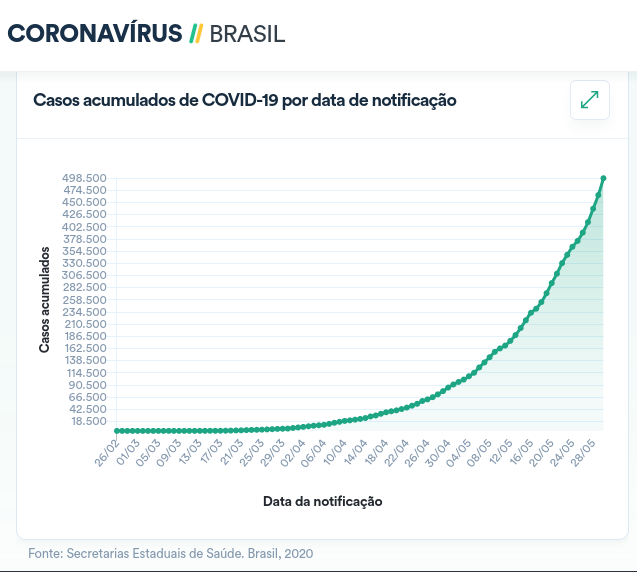
\includegraphics[width=400bp]{investigacao3}

\end{figure}

Ou ainda, para mostrar como evoluiu o índice de isolamento no Estado de São Paulo entre os meses de março e maio de 2020.

\begin{figure}[H]
\centering
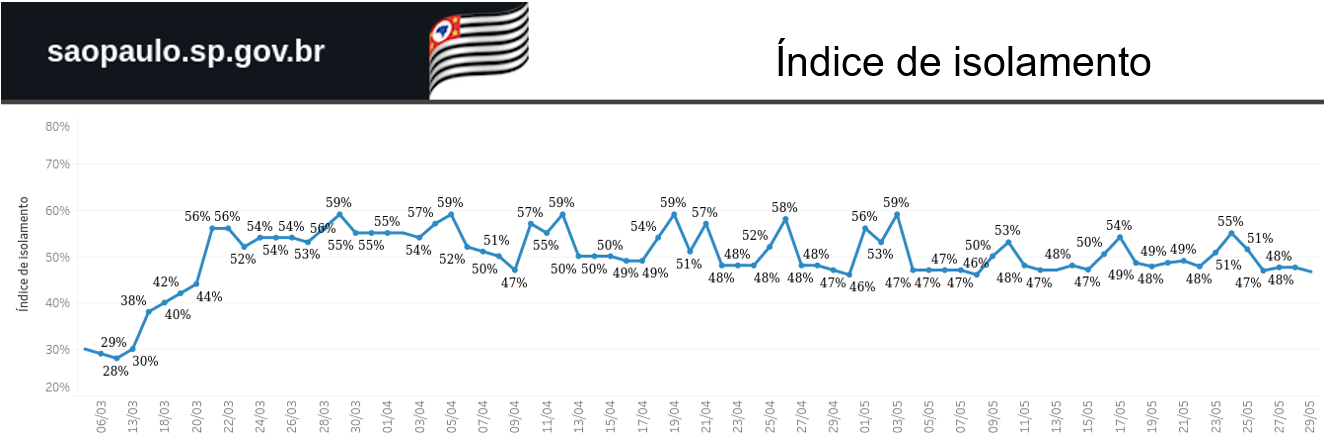
\includegraphics[width=400bp]{investigacao4}

\caption*{Fonte: Secretaria de Saúde do Estado de São Paulo. Acesso em 31/05/2020}
\end{figure}

Já os \textbf{gráficos de barras e colunas} são mais adequados para mostrar comparação entre quantidades. Um bom exemplo é o gráfico apresentado pelo Portal de Transparência de Registro Civil, que apresenta uma comparação da quantidade de óbitos com suspeita ou confirmação de COVID-19 por sexo e faixa etária.

\begin{figure}[H]
\centering
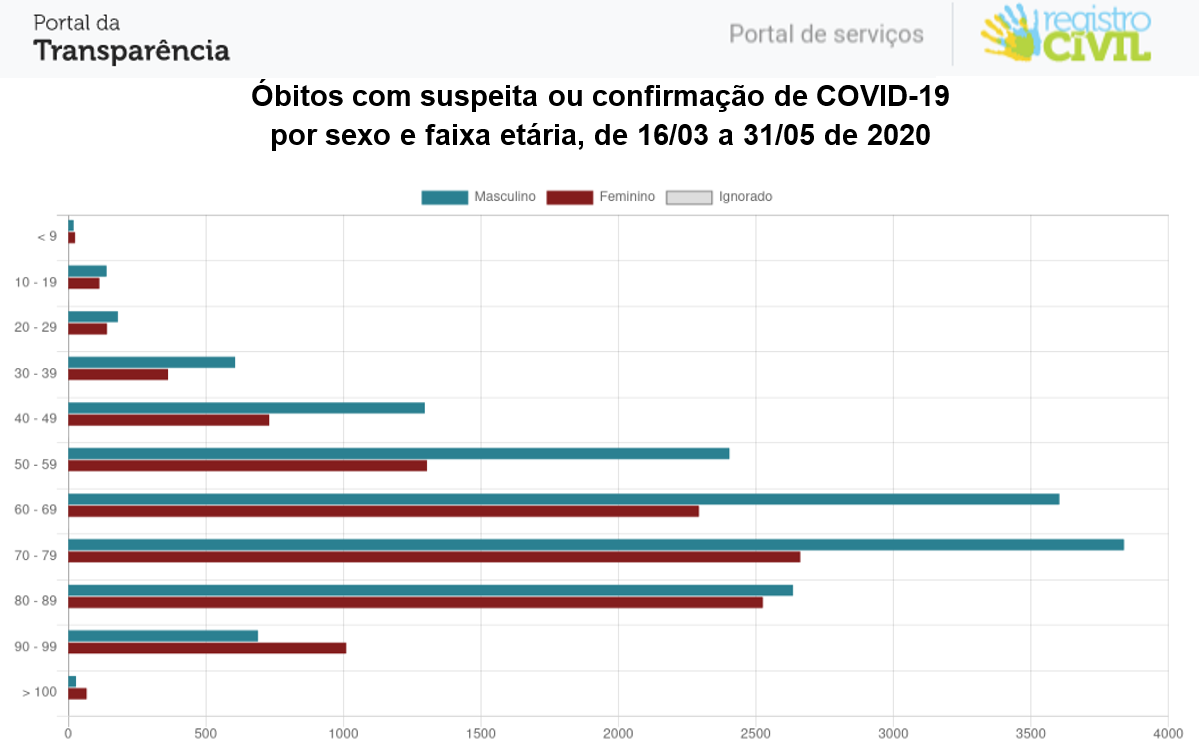
\includegraphics[width=400bp]{investigacao5}

\caption{Fonte: Central de Informações do Registro Civil - CRC Nacional}
\end{figure}

Os \textbf{gráficos de setores} dão noção de parte e todo, e por isso muitas vezes seus valores são apresentados na forma percentual. Esta foi a forma como o Estado de Santa Catarina escolheu para mostrar em seus boletins epidemiológicos a taxa de ocupação dos leitos de UTI. Repare como com este tipo de gráfico fica fácil entender se, comparado com o total de leitos, há muitos ou poucos livres.

\begin{figure}[H]
\centering
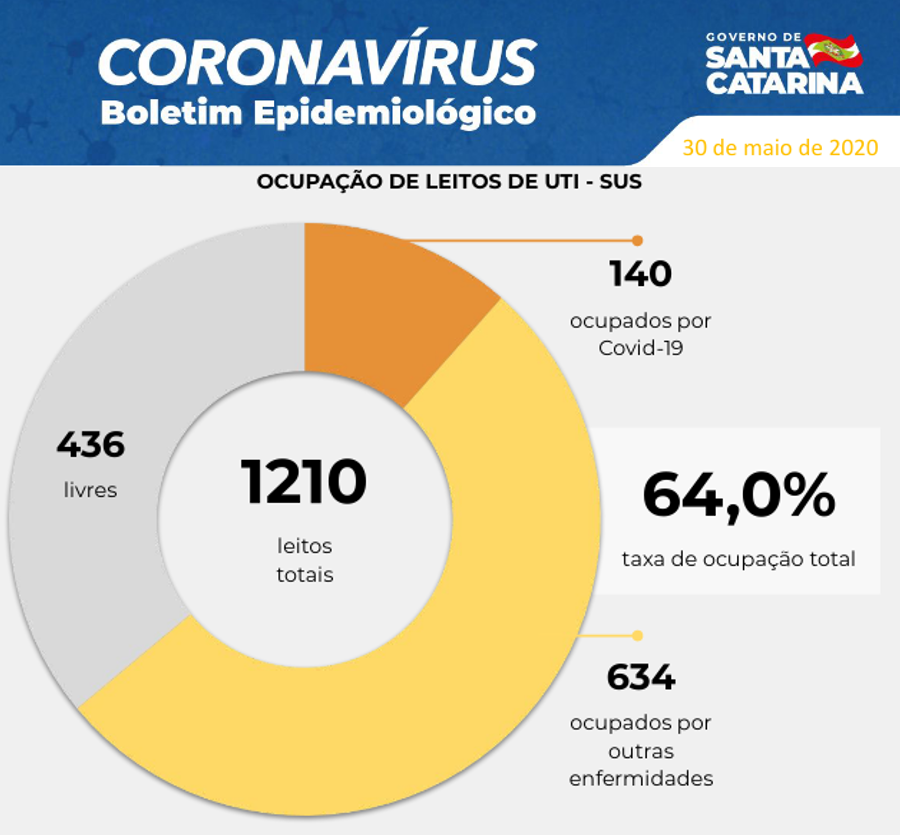
\includegraphics[width=290bp]{investigacao6}

\end{figure}


Existem muitas outras formas de mostrar dados quantitativos de formas visuais. Se você quiser se aprofundar um pouco mais neste assunto pode buscar também sobre as discussões a leitura e o uso de \textbf{infográficos} e \textbf{histogramas}, no capítulo introdutório do Livro de Estatística e Probabilidade do Livro Aberto, ou ainda uma discussão sobre a \textbf{representação gráfica de funções}, no capítulo introdutório do Livro de Funções do Livro Aberto. 

Com os programas de edição de imagem, hoje em dia até existe um profissional que é especializado em elaborar gráficos, tabelas e diagramas que ajudem os leitores a entenderem melhor as informações de uma certa notícia ou relatório. Para elaborar um bom gráfico é necessário conhecimento matemático, compreensão de qual informação quer-se enfatizar e muita criatividade!
\clearmargin
\def\currentcolor{session2}
\begin{texto}
{\vspace{-\baselineskip}
\subsection{Desenvolvendo a Investigação - Etapa 4}
(Tempo estimado 7-8 aulas)

\textbf{Objetivo geral}: Aplicar as ferramentas matemáticas para análise de uma situação concreta.

Esta é a etapa mais longa do projeto e por isso é necessária uma boa organização. Se os estudantes forem trabalhar com planilhas eletrônicas e arquivos compartilhados, é interessante criar um diretório para cada grupo, ao qual você tenha acesso à toda a produção deles. Se o trabalho for realizado sem computadores, uma boa solução é a utilização de um painel na sala para cada grupo ou simplesmente ir agrupando todas as fichas com planejamento, anotações e análises. É interessante que este material fique com o professor, para que se eventuais faltas não prejudiquem o trabalho coletivo. 

Uma estratégia interessante para organizar os avanços e próximos passos de cada grupo é o desenvolvimento do diário de bordo, que pode ser uma ficha ou arquivo digital, preenchido coletivamente pelos integrantes do grupo. 

É importante acompanhar o desenvolvimento dos grupos, para que eles não se percam. Uma estratégia válida é retomar periodicamente o documento de planejamento.

Também é importante garantir que todos os grupos apresentem seus resultados de múltiplas formas, utilizando texto, gráficos tabelas, etc… Certamente haverá grupos que finalizarão as análises antes. Estes grupos podem, por exemplo, investigar outras formas gráficas (mais elaboradas) de representar seus resultados, melhorando a comunicação de suas descobertas. Ou ainda, podem aprofundar sua investigação por outras perguntas correlacionadas que certamente surgirão ao longo da investigação. 

Haverá ainda grupos que não conseguirão chegar a um resultado final de sua investigação. Nesse caso é importante avaliar os motivos que fizeram com que o planejamento não funcionasse. Foi só uma questão de organização ou algum problema com os dados ou com a metodologia planejada para analisar os dados? Compreender o que não deu certo é uma boa forma de fazer com que o mesmo erro não se repita. Nesses casos, os resultados e as conclusões serão parciais. É possível que a conclusão seja simplesmente algo como “as análises e indicadores propostos não são uma boa forma de responder a pergunta escolhida”. Este tipo de conclusão também é válida, pois saber o que não funciona também é importante para responder uma pergunta. Por isso, esse tipo de resultado também deve ser valorizado.

Entre a terceira e quinta aula desta etapa, é importante, caso ainda não o tenha feito, apresentar  qual será o produto final deste projeto. Esta apresentação tem a finalidade de ajudar os estudantes a se organizarem e já irem montando seus resultados e conclusões num formato adequado para o produto final. Desta forma, é muito interessante que o educador entregue aos grupos um roteiro de produção do produto final. Exemplos de roteiros serão discutidos na próxima seção.

}
\end{texto}
\begin{example}{Planejamento da investigação - COVID-19}

Para as questões \titem{5} e \titem{6} do roteiro de organização da investigação, Rodrigo, Priscila e Thiago elaboraram os seguintes registros:

\begin{enumerate}[label=\titem{\arabic*)}]\setcounter{enumi}{4}
\item Expliquem como vocês utilizarão os dados para responder a pergunta investigativa do grupo. Dêem exemplos. Que cálculos vocês farão com esses dados e o que esperam obter? Não se esqueçam que ao final, a análise deve servir para testar a(s) sua hipótese(s) inicial(is).

\titem{Resposta}:\textit{Calcularemos as taxas de desocupação e iremos verificar a sua evolução ao longo do tempo. Por exemplo, no trimestre fev/mar/abr de 2019 a taxa era $12,5\%$, enquanto que em fev/mar/abr de 2020 era de $12,6\%$.  Assim, verificamos que a taxa de desocupação, nesta situação, não teve muita alteração. No entanto, nos questionamos sobre esses percentuais.}

\item Façam um esboço do(s) tipo(s) de gráfico(s) que vocês utilizarão para apresentar seus dados. Abusem das cores e criatividade em seu esboço. Não se esqueçam de identificar quais dados vocês esperam apresentar em cada gráfico que fizerem.

\begin{figure}[H]
\centering

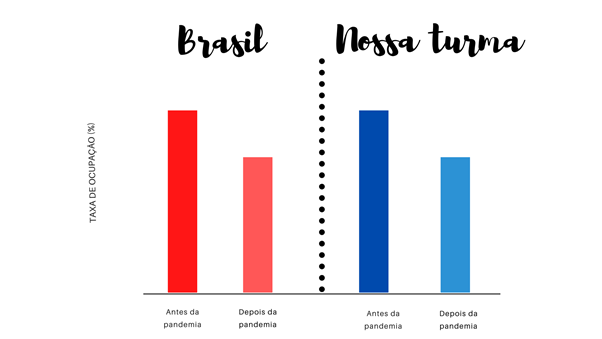
\includegraphics[width=\textwidth]{investigacao10}
\end{figure}

\end{enumerate}

\end{example}


\practice{Desenvolvendo a investigação - etapa 4}
\phantomsection\label{etapa4}

Agora é hora de colocar em prática o seu planejamento!

Mas antes de iniciar o trabalho pense sobre como organizá-lo. Onde os dados dos índices ficarão guardados? Onde você fará suas contas e seus gráficos? Vai utilizar um caderno ou uma planilha? Onde anotará novas fontes bibliográficas que for encontrado pelo caminho, seus resultados parciais e conclusões? Em trabalhos em grupo é necessário também pensar em estratégias para que todos tenha acesso a todos os dados, contas, resultados e conclusões. 

Uma boa estratégia é manter um diário de bordo no qual você escreve um pequeno parágrafo contando o que fez na aula, os avanços obtidos e os próximos passos. Este diário pode ser feito num caderno próprio ou ser um relato coletivo. 

As questões a seguir são uma síntese do que deve ser o seu resultado final. Você só conseguirá respondê-las quando finalizar sua pesquisa.

Mão à obra!

\begin{enumerate}
\item Como os indicadores, gráficos e tabelas que você construiu respondem a sua pergunta de investigação?
\item Você considera que os indicadores que você e seu grupo escolheram usar foram realmente adequados? Eles ajudaram a responder a pergunta investigativa de vocês? Justifique sua resposta.
\item Por último, escreva suas conclusões. É o resumo do que você aprendeu e do que se pode saber através desta investigação. Pode ser apenas uma frase e algumas vezes pode haver mais de uma conclusão. É muito importante que na conclusão você analise a sua hipótese inicial. Ela estava correta? Se não estava, o que os dados mostraram de diferente das suas expectativas iniciais?
\end{enumerate}

\clearpage
\begin{sugestions}{Exemplo: Realizando a investigação - COVID-19}
{
  O exemplo expressa uma simplificação da discussão que geralmente ocorre na sala de aula. Essas discussões, na realidade, são permeadas de dúvidas e de falas imprecisas. É saudável que as discussões sejam feitas em locais onde se possa consultar fontes, como em salas de informática, em biblioteca, ou que os próprios estudantes já tenham suas anotações e sínteses de pesquisas que já realizaram.

  É importante que o professor acompanhe algumas dessas discussões para perceber se as dúvidas e as respostas dadas a elas estão claras e se é necessário algum tipo de intervenção didática.

  Neste exemplo, é mostrada uma tabela que os estudantes conseguiram na plataforma Sidra, do IBGE. Esta plataforma contém informações de uma gama enorme de pesquisas do IBGE, e é interessante o professor dar uma olhada nela para poder orientar os estudantes sobre quais os dados pode obter por lá.

  Outro ponto interessante deste exemplo é a elaboração do questionário. Veja que é um questionário bem simples e procura atender bem objetivamente à pergunta formulada pelos estudantes. Outras informações, como o sexo, tipo de trabalho, remuneração, etc, poderiam ser incluídas com a finalidade de análises além das perguntas formuladas, mas deve se tomar cuidado para não tornar o questionário demasiado longo ou então tirar o foco da pergunta principal.

  Caso outras perguntas da turma tenham relação com esta, o questionário pode ser ampliado e as respostas podem ser aproveitadas por mais de um grupo. Por exemplo, se um grupo quiser investigar a inflação, a mudança dos salários e do poder de compra dos familiares de colegas, o questionário poderia ser ampliado com perguntas nesta direção.

}{1}{0}
\end{sugestions}
\begin{example}{Realizando a investigação - COVID-19}

Rodrigo, Priscila e Thiago acessaram o site do IBGE e buscaram os dados da PNAD Contínua\footnote{\url{https://www.ibge.gov.br/estatisticas/sociais/trabalho/9173-pesquisa-nacional-por-amostra-de-domicilios-continua-trimestral.html}}. Durante a pesquisa, perceberam que os relatórios apresentavam dados brutos e que poderiam, eles próprios, realizar os cálculos e fazer interpretações dos indicadores. Eles consultaram diversas tabelas no site do IBGE e chegaram na tabela 4092 do sistema SIDRA do IBGE\footnote{\url{https://sidra.ibge.gov.br/tabela/4092}}, onde fizeram alguns filtros e geraram a tabela a seguir.

\begin{figure}[H]
\centering

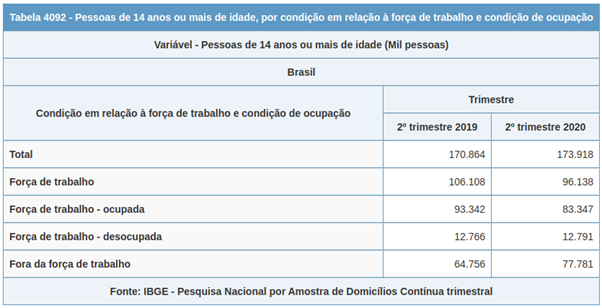
\includegraphics[width=\textwidth]{investigacao11}
\end{figure}

Em seguida deu-se a uma discussão sobre o que encontram
\begin{quote}
\textbf{Rodrigo}: Pessoal, reparei que o número de pessoas desocupadas no segundo trimestre de 2019 e no segundo trimestre de 2020 foi quase o mesmo.

\textbf{Thiago}: É verdade. Em compensação, o número de pessoas ocupadas diminuiu cerca de 10 mil pessoas.

\textbf{Priscila}: Você quis dizer 10 milhões de pessoas, certo, Thiago?

\textbf{Thiago}: Não. Eu quis dizer 10 mil mesmo. Na tabela tá dizendo que a força de trabalho ocupada era cerca de 93 mil pessoas e passou para 83 mil.

\textbf{Priscila}: Thiago, você esqueceu de ver que os números da tabela são em “milhares de pessoas”, como tá escrito na legenda. Quando a tabela coloca 93.342, ela não tá dizendo “93 mil pessoas”, mas sim “93 mil milhares de pessoas”. Quer dizer 93.342$\times$1000, ou seja, 93.342.000, que é cerca de 93 milhões de pessoas.

\textbf{Thiago}: Que confusão, Priscila! Mas eu entendi, você tem razão. E 93 mil pessoas realmente parece pouco mesmo, pois só na cidade onde moramos, que não é grande, tem cerca de 100 mil habitantes.

\textbf{Rodrigo}: Pessoal, voltando aos indicadores, acho que se queremos um indicador de pessoas ocupadas, não devemos apenas calcular o percentual de pessoas ocupadas dentro do total da força de trabalho. Acho que precisamos calcular com relação ao total de pessoas em idade de trabalhar. Veja que o número de pessoas em idade de trabalhar aumentou de 171 milhões para 174 milhões, mas o número de pessoas na força de trabalho diminuiu de 106 milhões de pessoas para 96 milhões.

\textbf{Priscila}: Tem razão. A impressão é que mais de 10 milhões de pessoas deixaram de trabalhar e passaram a integrar o grupo de pessoas “fora da força de trabalho”{} e não o grupo de “pessoas desocupadas”.

\textbf{Thiago}: Mas qual a diferença entre uma pessoa desocupada e uma pessoa fora da força de trabalho? Se ela está fora de força de trabalho, então ela não está desocupada?

\textbf{Priscila}: De certa forma, sim. Mas pelo que consultei no glossário do IBGE\footnote{\url{ftp://ftp.ibge.gov.br/Trabalho_e_Rendimento/Pesquisa_Nacional_por_Amostra_de_Domicilios_continua/Mensal/glossario_pnadc_mensal.pdf}}, eles usam o termo “força de trabalho” para se referir ao conjunto de pessoas que estão dispostas a trabalhar.

\textbf{Rodrigo}: Isso mesmo, e “desocupadas” são as pessoas na força de trabalho, isto é, que querem trabalhar, mas que não estão trabalhando por algum motivo, que pode ser por ter buscado mas não ter conseguido um trabalho, por falta de perspectiva em conseguir um emprego, ou por impossibilidade de assumir um emprego no momento.

\textbf{Priscila}: Isso mesmo. Pelo que parece muita gente deixou de trabalhar neste momento de pandemia.

\textbf{Thiago}: O que era de se esperar, né Priscila? Como trabalhar se precisamos ficar em casa para não propagar o coronavírus?

\textbf{Priscila}: Mas como ficar em casa se precisamos trabalhar para pagar nossas contas?

\textbf{Thiago}: Ta aí um grande dilema! Em todo caso,  o que parece é que muita gente não apenas parou de trabalhar, como também passou a ficar indisponível para trabalhar. Ou seja, essas pessoas deixaram a categoria de “ocupadas” e passaram para a categoria “fora da força de trabalho”.

\textbf{Rodrigo}: Ótima colocação, Thiago. Por isso penso que se queremos saber indicadores de emprego, não devemos apenas dividir o número de pessoas ocupadas pelo número de pessoas na força de trabalho, mas sim pelo número total de pessoas em idade de trabalhar.

\textbf{Priscila}: Pelo que pesquisei, Rodrigo, o IBGE também faz esse cálculo. Eles chamam de “nível de ocupação”.

\textbf{Thiago}: Nossa, quantas contas! Então a gente vai calcular “taxa de ocupação”, que é o percentual de pessoas ocupadas dentro do total da força de trabalho, e também o “nível de ocupação”, que é o percentual de pessoas ocupadas dentro do total de pessoas em idade para trabalhar.

\textbf{Rodrigo}: Sim, Thiago. Acho que é isso. Neste caso, as taxas se referem às pessoas na força de trabalho, isto é, que estão dispostas a trabalhar. Já o nível se refere ao total de pessoas em idade de trabalhar.
\end{quote}

Com essa decisão, o grupo elaborou a tabela a seguir com esses indicadores:

\begin{table}[H]
\centering

\begin{tabu} to \textwidth{|l|c|c|}
\hhline{~|--|}
\multicolumn{1}{c|}{} & \tcolor{\makecell{2$^{\circ}$ trimestre \\ 2019}} & \tcolor{\makecell{2$^{\circ}$ trimestre \\ 2020}} \\
\hline
Total (pessoas com 14 anos ou mais de idade) & 170.864* & 173.918* \\
\hline
(1) Taxa de participação na Força de Trabalho & $62{,}1\%$ & $55,\%$ \\
\hline
(2) Taxa de ocupação & $88{,}0\%$ & $86{,}7\%$ \\
\hline
(3) Taxa de desocupação & $12{,}\%$ & $13{,}3\%$ \\
\hline
Nível de ocupação [(1)$\times$(2)] & $54{,}6\%$ & $47{,}9\%$ \\
\hline
\end{tabu}
\flushright

\scriptsize{* em milhares de pessoas}
\end{table}

Além disso, com base nesses estudos, o grupo elaborou um questionário (instrumento de coleta) para saber a situação do emprego dentre os familiares dos colegas de classe. Para expressar as condições de ocupação, o grupo decidiu por três categorias: (a) pessoas ocupadas; (b) pessoas desocupadas mas com intenções de trabalhar e; (c) pessoas desocupadas sem intenções de trabalhar. As pessoas com idade igual ou superior a 14 anos integrantes nas categorias (a) e (b) formam o grupo “força de trabalho”, e as da categoria (c) estão “fora da força de trabalho”

\begin{center}
\framebox[.8\textwidth][c]
{\parbox{.75\textwidth}{
	\vspace{1em}
	\centering 
	\textbf{\large Questionário sobre trabalho e condição de ocupação}
	\justify

	\begin{enumerate}[label=\textbf{\arabic*. }, itemsep=0cm]
	\item Nome:
	\item Sexo:
	\item Idade:
	\item Em qual situação você se encontrava no 2$^{\circ}$ trimestre de 2019?
	\begin{enumerate}[label=(\alph*)]
	\item Estava ocupado
	\item Estava desocupado, mas tinha a intenção de trabalhar.
	\item Estava desocupado e nem tinha a intenção de trabalhar.
	\end{enumerate}
	\item Em qual situação você se encontrava no 2$^{\circ}$ trimestre de 2020?
	\begin{enumerate}[label=(\alph*)]
	\item Estava ocupado
	\item Estava desocupado, mas tinha a intenção de trabalhar.
	\item Estava desocupado e nem tinha a intenção de trabalhar.
	\end{enumerate}
	\end{enumerate}
	\flushright

	\textbf{Elaboradores}: Priscila, Rodrigo e Thiago
	\vspace{.5em}
	}

}
\end{center}
\end{example}
\clearpage
\begin{paginatexto}{Comunicando as Descobertas - Etapa 5}
\textit{(Tempo estimado 4-5 aulas)}

O objetivo específico desta seção é materializar todo o percurso desenvolvido e aprendizado adquirido pelo estudante durante a elaboração do projeto de investigação matemática. Dar concretude a este processo é importante pois, muitas vezes, ao trabalharmos com uma proposta aberta, com poucos momentos de sistematização e instrumentos conhecidos dos estudantes (como listas de exercícios e provas), os educandos têm dificuldade de perceber seu próprio aprendizado e precisam de um produto concreto para perceberem tudo o que evoluíram no processo. 
Além disso, ver o produto final de sua pesquisa concretizado é um momento de satisfação e orgulho para muitos dos estudantes, e de se perceberem como produtores de conhecimento, gerando um aumento na autoestima e no engajamento destes jovens. 

O produto final também é uma forma interessante de justificar e organizar o compartilhamento dos novos conhecimentos e descobertas que cada grupo fez durante o projeto de investigação. Este compartilhamento é de importância central, pois ajuda os estudantes a ampliarem seus repertórios e descobrirem os caminhos que os colegas tomaram para responderem suas próprias perguntas investigativas. E ainda, ajuda a criar uma atmosfera de comunidade, colaboração, troca de saberes na turma. Este processo é interessante porque ajuda a desconstruir a ideia de que o professor é o único detentor de conhecimento e, por isso, o único que precisa ser ouvido, possibilitando a construção de um espaço mais democrático no que tange à valorização das vozes na sala de aula. 

Algumas possibilidades de produtos finais são:

\begin{itemize}
\item uma revista “científica” com os artigos dos grupos;
\item um congresso com um seminário de cada “grupo de pesquisa”;
\item uma série de podcasts, no qual cada grupo faz o seu programa;
\item um telejornal ou um canal com vídeos de cada grupo;
\item uma página de internet para cada grupo apresentar suas descobertas sobre o tema estudado;
\item um fanzine ou uma história em quadrinhos (HQ);
\item um panfleto ou um folder.
\end{itemize}

Entretanto, há uma infinidade de outras opções e o educador é livre para escolher o produto que mais sentido fizer para si, sua realidade e sua comunidade escolar. 

A definição do tema de investigação e do produto final no qual a pesquisa se materializará estão intimamente relacionados e devem ser escolhidos de forma a se complementarem. Além disso, a definição tanto do tema, quanto do produto final, depende do contexto e inquietações da comunidade escolar. Dentro do contexto, para pensar o produto final, é importante levar em conta o s recursos físicos e tecnológicos da unidade escolar. Por exemplo, não é adequado pensar na produção de uma revista científica ou vídeos para um canal de Youtube em uma escola na qual os estudantes não têm acesso regular aos computadores. Mas para esses casos há inúmeras outras possibilidades, como fanzines, um congresso ou até mesmo uma ação comunitária com a comunidade da região na qual a escola está inserida. 

Um ponto de atenção nesse processo é que o produto final não deve se focar apenas na resposta encontrada para a pergunta investigativa do grupo, mas também no caminho percorrido pelos estudantes para chegarem em sua resposta. Em outras palavras, o produto final deve contar tanto o “o quê aconteceu” como o “como aconteceu”.

Como já explicitado anteriormente, a escolha do produto final deve ser feita antes do projeto se iniciar e um roteiro orientador para a produção do produto final deve ser entregue ainda no início da etapa de desenvolvimento da investigação. Estas informações ajudam o estudante a manter-se orientado, com foco em algo concreto. 

Durante este processo é interessante que os estudantes percebam que a forma da comunicação muda de acordo com o produto. Isto é, um texto para ser publicado em uma revista científica é diferente de um texto de história em quadrinhos, que é diferente de um texto de fanzine. Uma possibilidade muito interessante é trabalhar o produto final em parceria com outra(s) disciplina(s). Em muitos casos as disciplinas de português e artes podem ser grandes aliadas nesse processo. 

\subsection{Sugestões e Discussões: Refletindo sobre o produto final}

As questões apresentadas aos estudantes nessa seção tem a finalidade de ajudá-lo a refletir sobre o que é importante para produzir um bom produto final. Para isso, ele deve pensar sobre quem é seu público alvo, qual é a linguagem mais adequada para esse público e para o tipo de produto final que ele irá fazer e quais as informações que não podem deixar de estar presentes neste produto final. Todas essas questões variam de acordo com o tipo de produto.

Por exemplo, a revista científica é um tipo de comunicação que surgiu para que cientistas pudessem se comunicar entre si, com uma proposta de comunicar suas descobertas e validá-las com seus pares. Desta forma, em um produto final do tipo revista científica é necessário ter em mente que os leitores devem ser capazes de reproduzir os resultados obtidos pelo grupo. Assim, neste tipo de produto final, deve haver um texto extenso sobre os cálculos e análises realizados para se chegar nos resultados obtidos. Por outro lado, os fanzines são publicações de baixo custo, que surgiram com o movimento político atrelado ao punk. A proposta era difundir ideias de forma barata, aumentando sua abrangência. Sua produção pode ser feita a partir de uma matriz original toda a mão, que, quando pronta, é fotocopiada (xerocada) e distribuída. Neste tipo de produto final, há uma maior liberdade editorial e a proposta pode ser a de alertar a comunidade escolar para as descobertas obtidas pelos grupos, sem se preocupar em passar para os leitores o rigor metodológico. Uma terceira possibilidade poderia ser uma peça de teatro ou a composição de uma música com os resultados das investigações. Cada um desses exemplos de produtos finais demanda um tipo de linguagem diferente, que dá sentido a certas formas de expressão. 

A reflexão sobre a forma de expressão e linguagem apropriada ao produto final deve ser realizada com os estudantes antes deles iniciarem o processo de produção de seus produtos finais. Assim, é interessante que, após ser realizada uma conversa inicial sobre as principais características do produto final escolhido e dos estudantes responderem as perguntas reflexivas (colocadas como atividades nesta seção do livro do estudante), seja retomado o roteiro orientador do produto final, entregue para os educandos no início da etapa anterior. Exemplos de um roteiro orientador para a produção de artigos científicos e outro para a produção de fanzines pode ser encontrada no \hyperref[roteiro-artigo]{final do capítulo}. 

Perceba que os roteiros são bem diferentes e o trabalho para a produção de cada um desses textos também o é. No caso do artigo científico é recomendado que os estudantes possam escrever os artigos no computador e produzam gráficos em planilhas. Já no caso do fanzine, o ideal é fazer tudo a mão, num processo de colagem, com uma boa discussão sobre a ocupação do espaço da página. 

O mais importante é que o produto final seja realmente uma boa forma de comunicação e compartilhamento das descobertas dos diferentes grupos. Por isso, a atividade de compartilhamento também se altera de acordo com o produto final. No caso de produtos na forma de revistas, como a revista científica e o fanzine, uma opção é fazer uma aula de leitura e discussão dos textos. Já no caso dos podcasts e vídeos, uma atividade de exibição com roda de discussão é uma ótima possibilidade. 
\clearpage
\end{paginatexto}

\practice{Comunicando as descobertas - etapa 5}
\phantomsection\label{etapa5}

Agora é hora de materializar todo o aprendizado do grupo em um produto final. As possibilidades são ilimitadas e dependem da criatividade e de recursos (como tempo para execução, acesso a computadores e internet, disponibilidade de material papel e tinta, etc). 

Algumas possibilidades são:

\begin{itemize}
\item um revista "científica"{}com os artigos dos grupos;
\item um congresso com um seminário de cada "grupo de pesquisa";
\item uma série de podcasts no qual cada grupo faz o seu programa;
\item um telejornal ou um canal com vídeos de cada grupo;
\item uma página de internet para cada grupo apresentar suas descobertas sobre o tema estudado;
\item um fazine ou uma história em quadrinho (HQ);
\item um panfleto ou um folder;
\end{itemize}

\begin{task}{refletindo sobre o produto final}

Vamos pensar um pouco sobre o que é important que haja nesse produto final. Realize em uma ficha ou em seu caderno os registros para as questões a seguir.

\begin{itemize}
\item Pesquise e discuta com colegas quais as principais características do tipo de produto final escolhido para ser realizado como finalização deste projeto de investigação. Registre em uma ficha ou em seu caderno os pontos de atenção para produzir um bom produto final.
\item Quem é o público alvo de seu produto final?
\item Quais são as informações mais importantes de sua investigação. Isto é, o que seu público alvo precisa aprender com seu produto final?
\end{itemize}

Agora é hora de efetivamente dar vida ao produto final. Após ele ficar pronto e ser compartilhado com seus colegas. Volte para responder às últimas pergutnas desta Unidade Temática.

\begin{itemize}
\item Como foi ver o seu produto final concretizado? O que você sentiu? O que acha que ficou bom e o que poderia ser melhorado?
\item O que você sente que aprendeu durante todo esse processo de investigação?
\item O que você achou de toda essa experiência?
\end{itemize}
\end{task}

\ifnum\aluno=1
\else
\cleardoublepage
\phantomsection\label{avaliacoes}
\def\currentcolor{session1}
\centering
\textbf{\Large\color{\currentcolor} Roteiro de autoavaliação após etapa de planejamento}
\justify
A tabela a seguir é um guia para você pensar no percurso que você fez para planejar a sua investigação. Assinale as alternativas de acordo com sua participação individual nesta etapa do trabalho em grupo.

\begin{table}[H]
\centering
\begin{tabu} to \textwidth{|>{\vspace{2.5pt}}m{.6\textwidth}<{\vspace{2.5pt}}|c|c|c|}
\hline
\thead
& SIM & NÃO & EM PARTE \\
\hline
1. Eu estive presente nas aulas? & & & \\
\hline
2. Eu colaborei com ideias para o grupo? & & & \\
\hline 
3. Eu consegui ouvir as ideias do meu grupo? & & & \\
\hline
4. Eu colaborei para resolver conflitos e discordâncias no grupo? & & & \\
\hline
5. Eu ajudei na elaboração da hipótese inicial, de forma que ela represente meu pensamento? & & & \\
\hline
6. Eu ajudei a selecionar bons indicadores, fontes de informações seguras e tipos de gráficos adequados? & & & \\
\hline
7. Estou seguro quanto ao caminho que escolhemos para responder nossa pergunta e concordo com o planejamento do meu grupo. & & & \\
\hline
\end{tabu}
\end{table}


Levando em conta suas respostas na tabela anterior, avalie seu próprio desempenho (em inadequado, adequado e destaque) nos quesitos da tabela a seguir.  

\begin{table}[H]
\centering

\begin{tabu} to \textwidth{|l|c|c|}
\hline
\thead
& ESTUDANTE & PROFESSOR \\
\hline
Qualidade do planejamento & & \\
\hline
Colaboração com o grupo & & \\
\hline
\end{tabu}
\end{table}

Levando em conta tudo o que aconteceu nesta etapa, anote:
\begin{itemize}[itemsep=4em]
\item Uma coisa que aprendeu com seus colegas;
\item Algo que você ainda não entendeu;
\item Uma atitude que você pode melhorar para a próxima etapa.
\end{itemize}
\cleardoublepage

\centering
\textbf{\Large\color{\currentcolor} Ficha de reflexão para uma aula do praticando}\footnote{Ficha adaptada de \citet{boaler2018}}
\justify

Apesar de estarmos realizando um trabalho em grupo, é muito importante que cada estudante reflita sobre seu percurso e aprendizado individual. As questões a seguir têm o objetivo de te ajudar neste processo. Responda-as pensando bem sobre como a aula de hoje foi para você!

{\noindent Qual foi a principal ideia que discuti com meu grupo na aula de hoje?
\setlength\parskip{6em}

\noindent O que aprendi hoje?

\noindent Quais boas ideias tive hoje?

\noindent Em que situações eu poderia usar o conhecimento que aprendi hoje?

\noindent Que dúvidas tenho sobre o trabalho que fiz hoje com meu grupo?

\noindent Sobre quais novas ideias a atividade de hoje me fez pensar?
}

\cleardoublepage

\centering
\textbf{\Large\color{\currentcolor} Avaliação --- Produto Final}
\vspace{3em}

\flushleft
Nome:\makebox[20em]{\hrulefill}

Data:\makebox[10em]{\hrulefill}

\vspace{5em}
\justify
\begin{figure}[H]
\centering

\resizebox{\textwidth}{!}{
\begin{tikzpicture}[every node/.style={scale=.8}, scale=.75]
\foreach \x in {1,...,4} \draw circle (\x);

\foreach \x/\y/\z in {
0/{Considero que o produto final tem qualidade}/right,
45/{Colaborei na escrita do produto final}/above right,
90/{Colaborei na escolha de informações para o produto final}/above,
135/{Consegui colocar minhas ideias para o grupo}/above left,
180/{Consegui ouvir as ideias do meu grupo}/left,
225/{Entendo todo o processo que foi realizado, desde a elaboração da pergunta, até a produção do produto final}/below left,
270/{Ajudei a responder as duvidas dos colegas no momento de compartilhamento}/below,
315/{Compreendo a importância de adaptar a comunicação ao público alvo}/below right}
\draw (0,0) -- (\x:5) node [pos=1,\z] {\parbox[.5cm]{4.5cm}{\y}};

\end{tikzpicture}}
\end{figure}


\cleardoublepage
\phantomsection\label{relatorio-individual}
\centering
\textbf{\Large\color{\currentcolor} Roteiro de redação de relatório individual}
\justify

Relatórios são importantes ferramentas de registro e divulgação de resultado e ideias. Neles, as etapas de desenvolvimento de uma ideia ou projeto são relatadas de forma organizada, muitas vezes evidenciando a visualização de resultados, retomada de procedimento e comparação de dados. 

Nesse projeto, o relatório é importante para:

\begin{itemize}
\item Organizar o pensamento;
\item Entender e análisar fenômenos;
\item Sistematização do aprendizado;
\item Instrumento de avaliação.
\end{itemize}

Um relatório  deve ser organizado em etapas, bem identificadas e detalhadas:
\setlength\parskip{1.5em}

\noindent\textbf{Identificação}: Todo relatório deve ser identificado com nome do autor (você), data e disciplina.

\noindent\textbf{Título}: Todo relatório deve ter um título informativo. O título não pode ser “Relatório de matemática”, deve conter uma informação que identifique o assunto do qual o relatório trata.

\noindent\textbf{Introdução}: É o momento em que é apresentado o tema e objetivo do projeto de uma forma geral. A introdução deve apresentar qual era a pergunta e as hipóteses do grupo. Pode ser escrito em um parágrafo.

\noindent\textbf{Análise dos dados e resultados}:  É o passo a passo. Você deve explicar quais as técnicas que utilizou para analisar os dados que coletou. É importante prestar atenção, pois nessa etapa deve ser escrito o “como foi feito” e não “o que isso explica”. 

\noindent\textbf{Explicação dos resultados ou Discussão dos resultados}: Aqui você deve explicar os resultados de suas análises. É o “o que isso explica”.  Não se esqueça de comparar seu resultado com sua hipótese inicial.

\noindent\textbf{Conclusão}: É o resumo do que você aprendeu o do que se pode saber por meio  desta investigação. Pode ser apenas uma frase e algumas vezes pode haver mais de uma conclusão.

\noindent\textbf{Referências bibliográficas}: Devem ser listadas todas as fontes (livros, revistas científicas, sites) consultadas e utilizadas na explicação dos resultados, introdução ou em outra parte do relatório. Para livros e revistas científicas você deve colocar o nome do livro/revista, ano de publicação, autor, editora e volume (se tiver). Em caso de sites o endereço deve ser escrito por inteiro e constar autor, título do artigo e a data de acesso.

\noindent\textbf{O RELATÓRIO SEMPRE DEVE SER FEITO EM FOLHA SEPARADA E COM BOA APRESENTAÇÃO (LIMPO, NÃO AMASSADO E EM FOLHA DE MONOBLOCO).}

\cleardoublepage

\phantomsection\label{elaboracao-questoes}
\centering
\textbf{\Large\color{\currentcolor}Ficha de elaboração de questões}
\justify

Elabore três perguntas investigativas sobre aspectos do tema de investigação da turma. Tente seguir os critérios mencionados. Utilize as atividades disparadoras. Ao fazer as atividades propostas, quais curiosidades e questionamentos vêm à sua mente?

Uma dica: Ao pensar em perguntas tente imaginar como você faria para respondê-las. Que tipo de dados, medidas ou observações seriam necessárias? Se você não souber por onde começar, provavelmente você pensou em uma pergunta é complexa.

\setlength\parindent{0em}
\parbox{\linewidth}
{
  1. \hrulefill\\

  \hrulefill\\

  \hrulefill\\
}

\parbox{\linewidth}
{
  2. \hrulefill\\

  \hrulefill\\

  \hrulefill\\
}

\parbox{\linewidth}
{
  3. \hrulefill\\

  \hrulefill\\

  \hrulefill\\
}

Agora é hora de definir qual será a sua pergunta de investigação.

Escreva no quadro abaixo a pergunta na qual você irá se aprofundar. Lembre-se que ela tem que atender a todas as características discutidas no texto “O que é uma boa pergunta científica”.

\newtcolorbox{stretchbox}[1][]{
  height fill,
  sharp corners,
  colback=white,
  colframe=black,
  #1}

  \begin{stretchbox}
  \centering
  \textbf{\Large Minha proposta de questão investigativa}
  \end{stretchbox}

  \cleardoublepage
\phantomsection\label{roteiro-artigo}
\centering
\textbf{\Large\color{\currentcolor} Roteiro de redação do artigo científico}
\justify
\setlength\parindent{0em}

Os artigos científicos devem conter:
\setlength\parskip{1.5em}

\noindent\textbf{Título}

\noindent\textbf{Autores}

\noindent\textbf{Instituição}

\noindent\textbf{Resumo}: É um spoiler. A função do resumo é o leitor saber se aquele artigo tem o que ele procura. Então nesta seção deve estar contida a pergunta de investigação, o(s) índice(s) analisado(s) e as conclusões.

\noindent\textbf{Palavras-chave}: São as \textit{hashtags}. O ideal é colocar entre 3 e 4 palavras ou termos chaves

\noindent\textbf{Introdução}:  Nela devem estar contidas as seguintes informações:qual é a pergunta, por que ela é interessante, como ela se insere no conhecimento científico da área, quais as hipóteses iniciais que vocês tinham e como pretendem verificá-las.

\textbf{Coleta e análise de dados}: Esta seção deve apresentar os procedimentos de coleta e dados utilizados, os procedimentos de análise dos dados, os  resultados obtidos e uma discussão dos resultados que dialoga com as hipóteses iniciais de vocês.

\textbf{Conclusão}: Nela deve ser apresentado o resumo do que você aprendeu o do que se pode saber através desta investigação. Pode ser apenas uma frase e algumas vezes pode haver mais de uma conclusão. É muito importante que na conclusão você analise a sua hipótese inicial. 

\textbf{Bibliografia}


\cleardoublepage
\centering
\textbf{\Large\color{\currentcolor} Roteiro de redação do fanzine}
\justify

Cada grupo terá o espaço de duas páginas para comunicar os pontos mais relevantes de sua investigação. Neste texto deve haver:
\setlength\parindent{0em}

\textbf{Título}

\textbf{Autores}

\textbf{Dados}: Quais os dados que serão comunicados? Como eles vão aparecer? No texto? Em tabela? Em gráfico? Como serão explicados?

\textbf{Texto}: O texto deve mostrar para o leitor por que esse tema é interessante e /ou relevante. Também deve conter a(s) principal(is) descoberta(s) do grupo e dar um significado mais concreto para ela(s).

\textbf{Imagem}: Junto com o texto deve haver uma imagem que se conecte intimamente ao assunto texto. Pode ser um gráfico, uma foto, um desenhos… Lembre-se apenas de que ela será preto e branca.

\textbf{Destaque}:
Qual é a informação de destaque desse texto e como ela vai aparecer na página?

\textbf{Layout}:
Num fanzine é muito importante pensar no desenho da página, que chamamos de layout do texto. Para isso é importante pensar nas seguintes questões: Onde vai ficar a imagem? Quanto de espaço das páginas o texto ocupará? Onde ficará o título? As letras serão grandes ou pequenas?


Dica: vocês podem fazer todas as partes em em uma folha,  recortá-las e ir montando (como um quebra cabeças) nas duas páginas do fanzine. Quando acharem o layout ideal, colem as partes. A matriz das páginas do grupo  estará pronta!

\fi

\ifnum\aluno=1
\clearpage
\else
\notasfinais
\fi

\bibliographystyle{apalike-pt}
\bibliography{../Bibliografia/investigacao_bibliografia.bib}

\nocite{*}